
\documentclass{beamer}

% 字符编码设置
\usepackage[utf8]{inputenc}

% 引号格式 (csquotes)
\usepackage{csquotes}

% 数学和字体设置
\usepackage{newtxtext,newtxmath}
\usepackage{amsmath}

\usepackage{hyperref} % link

% 图形相关宏包
\usepackage{graphicx}
\usepackage{animate}  % 用于动画支持
\usepackage{epstopdf} % 如果使用 EPS 图片
%\usepackage{subfigure} % 已废弃,建议使用 subcaption 代替
\usepackage{subcaption}

% 表格和调整工具
\usepackage{array}
\usepackage{booktabs}
\usepackage{adjustbox}  % 调整表格或图片的大小

% 绘图工具 (tikz)
\usepackage{tikz} % 在幻灯片中用于绘制图形或箭头

% Beamer 主题设置
\usetheme{Warsaw}

% 自定义颜色设置
\definecolor{customcolor}{RGB}{25,54,120}
\usepackage{xcolor} %color in the formula

% 应用自定义颜色到不同的 Beamer 部分
\setbeamercolor{palette primary}{bg=customcolor}
\setbeamercolor{palette secondary}{bg=customcolor}
\setbeamercolor{palette tertiary}{bg=customcolor}
\setbeamercolor{palette quaternary}{bg=customcolor}
\setbeamercolor{section in head/foot}{bg=customcolor}


% \usepackage{tikz}

% \setbeamertemplate{footline}{%
%   \leavevmode%
%   \hbox{%
%   \begin{beamercolorbox}[wd=.5\paperwidth,ht=2.25ex,dp=1ex,left]{author in head/foot}%
%     \usebeamerfont{author in head/foot}\insertshortauthor~~(\insertshortinstitute)
%   \end{beamercolorbox}%
%   \begin{beamercolorbox}[wd=.5\paperwidth,ht=2.25ex,dp=1ex,right]{title in head/foot}%
%     \usebeamerfont{title in head/foot}\insertshorttitle\hspace*{2em}
%     \insertframenumber{} / \inserttotalframenumber\hspace*{2ex}
%   \end{beamercolorbox}}%
%   \vskip0pt%
% }
% \addtobeamertemplate{footline}{%
%   \begin{tikzpicture}[remember picture,overlay]
%     \node[anchor=south east,yshift=2ex] at (current page.south east) {\includegraphics[height=1cm]{jhu-logo.png}};
%   \end{tikzpicture}%
% }{}

\title{Pancreatic Duct Flows for a Novel Non-invasive Diagnosis of Chronic Pancreatitis }
\author{Haobo Zhao}
\date{\today}

\begin{document}

\frame{\titlepage}







% Page - Introduction  %%%%%%%%%%%%%%%%%%%%%%%%%%%%%%%%%%%%%
\begin{frame}
    \fontsize{8pt}{10pt}\selectfont
    \frametitle{ Introduction }

    Chronic pancreatitis (CP) which results in  
    debilitating abdominal pain can be caused 
    by pancreatic ductal (PD) hypertension (PDH) 
    or  from  neuropathy. 

    \begin{columns}
        \begin{column}{0.4\textwidth}

            \begin{figure}[H]
                \centering
                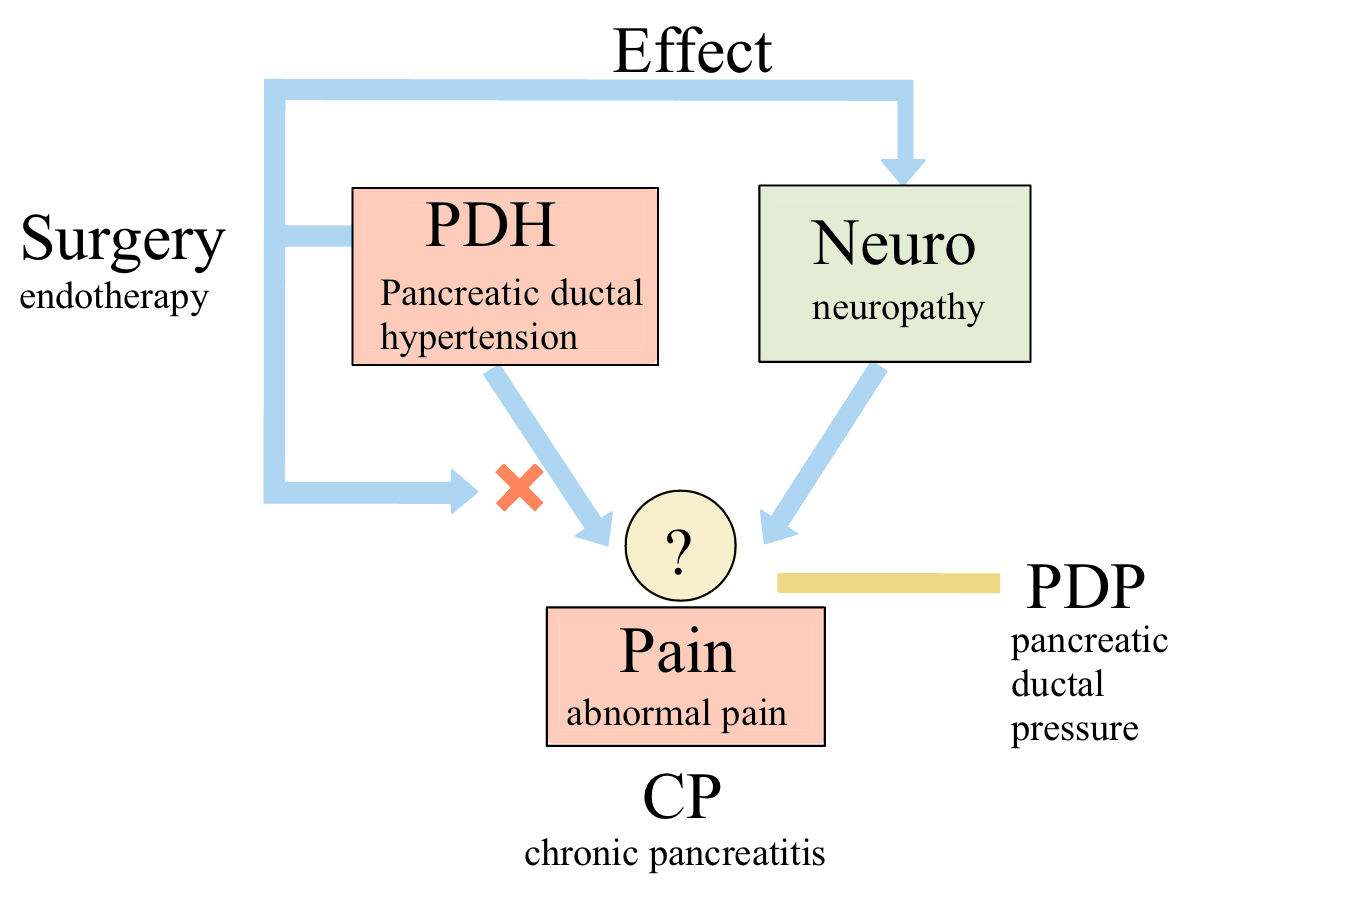
\includegraphics[width=1.2\textwidth]{figures/Introduction.jpg}
                % \caption{\scriptsize{Total_Process}}
            \end{figure}

                        
            Surgery could relieve PDH, but will
            effect neuropathic pancreatitis.

            \vspace{0.02\textwidth}

            Need to measure 
            pancreatic ductal pressure (PDP)
            to limit endotherapy to patients 
            have PDH

        \end{column}

        \hspace{0.05\textwidth}


        \begin{column}{0.65\textwidth}
            \vspace{0.1\textwidth}

            % \begin{small}
                \centering{PDP measurements:}
            % \end{small}

            \vspace{0.02\textwidth}
            \begin{columns}

                \begin{column}{0.5\textwidth}
        
                    \centering{\textbf{Traditional Way: ERCP}}
        
                    \begin{figure}[H]
                        \centering
                        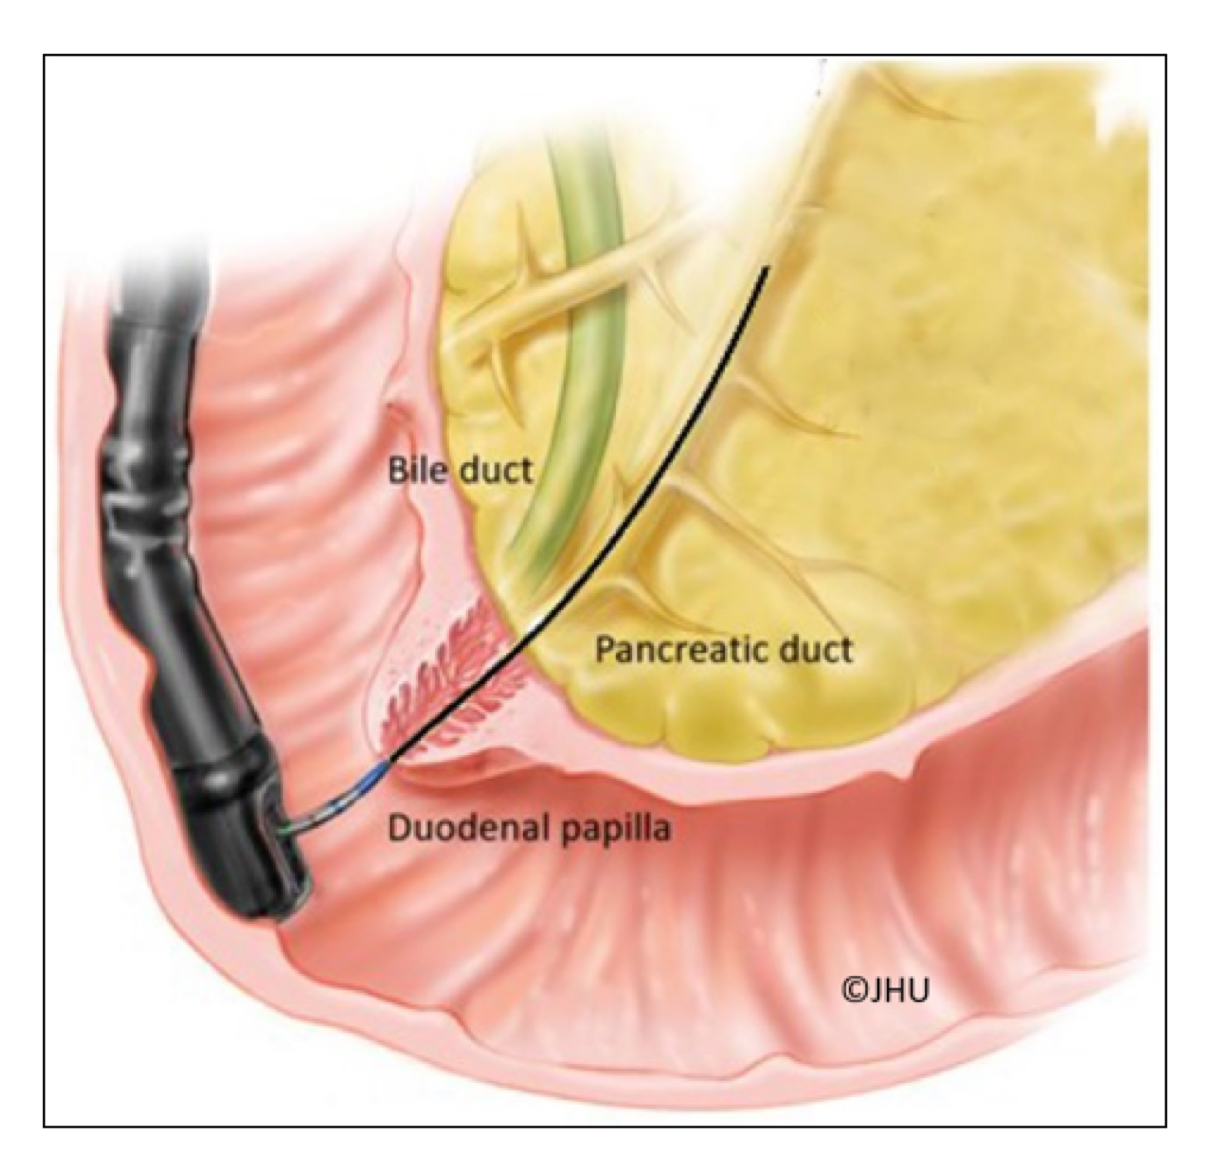
\includegraphics[width=0.6\textwidth]{figures/ERCP.jpg}
                        % \caption{\scriptsize{Total_Process}}
                    \end{figure}
                \end{column}

                \hspace{-0.15\textwidth}
                    
                
                    \begin{column}{0.5\textwidth}
        
                        \centering{\textbf{New Method: MRCP}}
            
                        \begin{figure}[H]
                            \centering
                            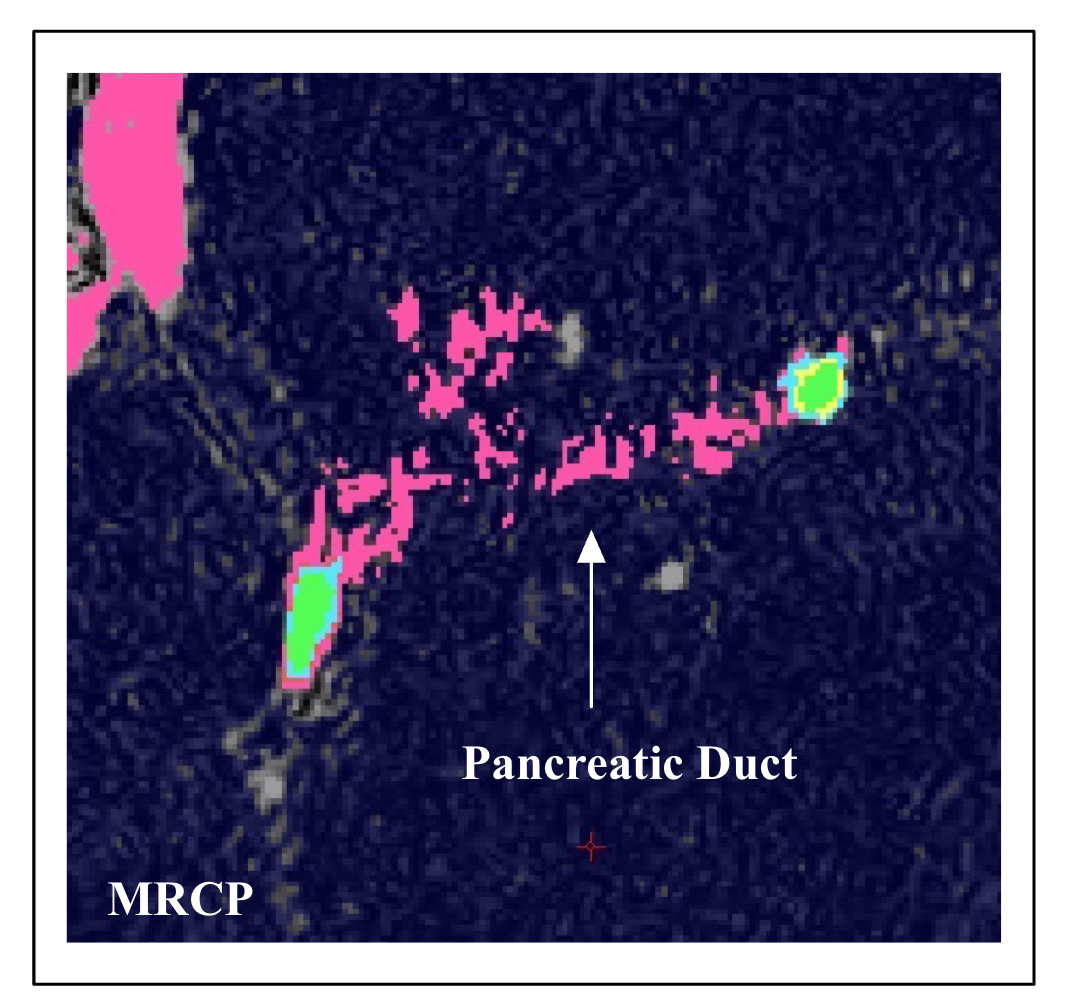
\includegraphics[width=0.6\textwidth]{figures/MRCP_0.jpg}
                            % \caption{\scriptsize{Total_Process}}
                        \end{figure}
                    \end{column}
                \end{columns}
                    
        
                \begin{columns}
        
                    \begin{column}{0.5\textwidth}
                    \begin{itemize}
                        \item \textbf{Invasive procedures}
                        \item Costly
                        \item Significant health risks 
                    \end{itemize}   
                    
                \end{column}

                \hspace{-0.15\textwidth}
                
        
                
                
                \begin{column}{0.5\textwidth}
        
                    \begin{itemize}
                        \item \textbf{Non-invasive approach}
                        \item Improve diagnostic accuracy 
                        \item Reduce patient exposure to harmful procedures
                    \end{itemize}   
                    
                \end{column}
            \end{columns}
        

            
        \end{column}
    \end{columns}

    % \vspace{0.05\textwidth}


    

\end{frame}






% Page - Pipeline: From MRI to CFD Simulation  %%%%%%%%%%%%%%%%%%%%%%%%%%%%%%%%%%%%%
\begin{frame}
    \fontsize{8pt}{10pt}\selectfont
    \frametitle{Pipeline: From MRI to CFD Simulation }
    \vspace{0.02\textwidth}

    \begin{columns}
        \begin{column}{0.6\textwidth}
            In order to investigate the correlation between PD pressure and abdominal pain, 
            patient-specific image-based CFD analysis of PD flows has been performed.
            
            \vspace{0.02\textwidth}


            \begin{itemize}
                \item   3D model of the PD is reconstructed from: magnetic resonance cholangiopancreatography (MRCP)
                \item Simulation is performed to determine the flow pattern and measure the pressure drop across the duct.
            \end{itemize}

            
            
        \end{column}

        \begin{column}{0.4\textwidth}

            \begin{figure}[H]
                \centering
                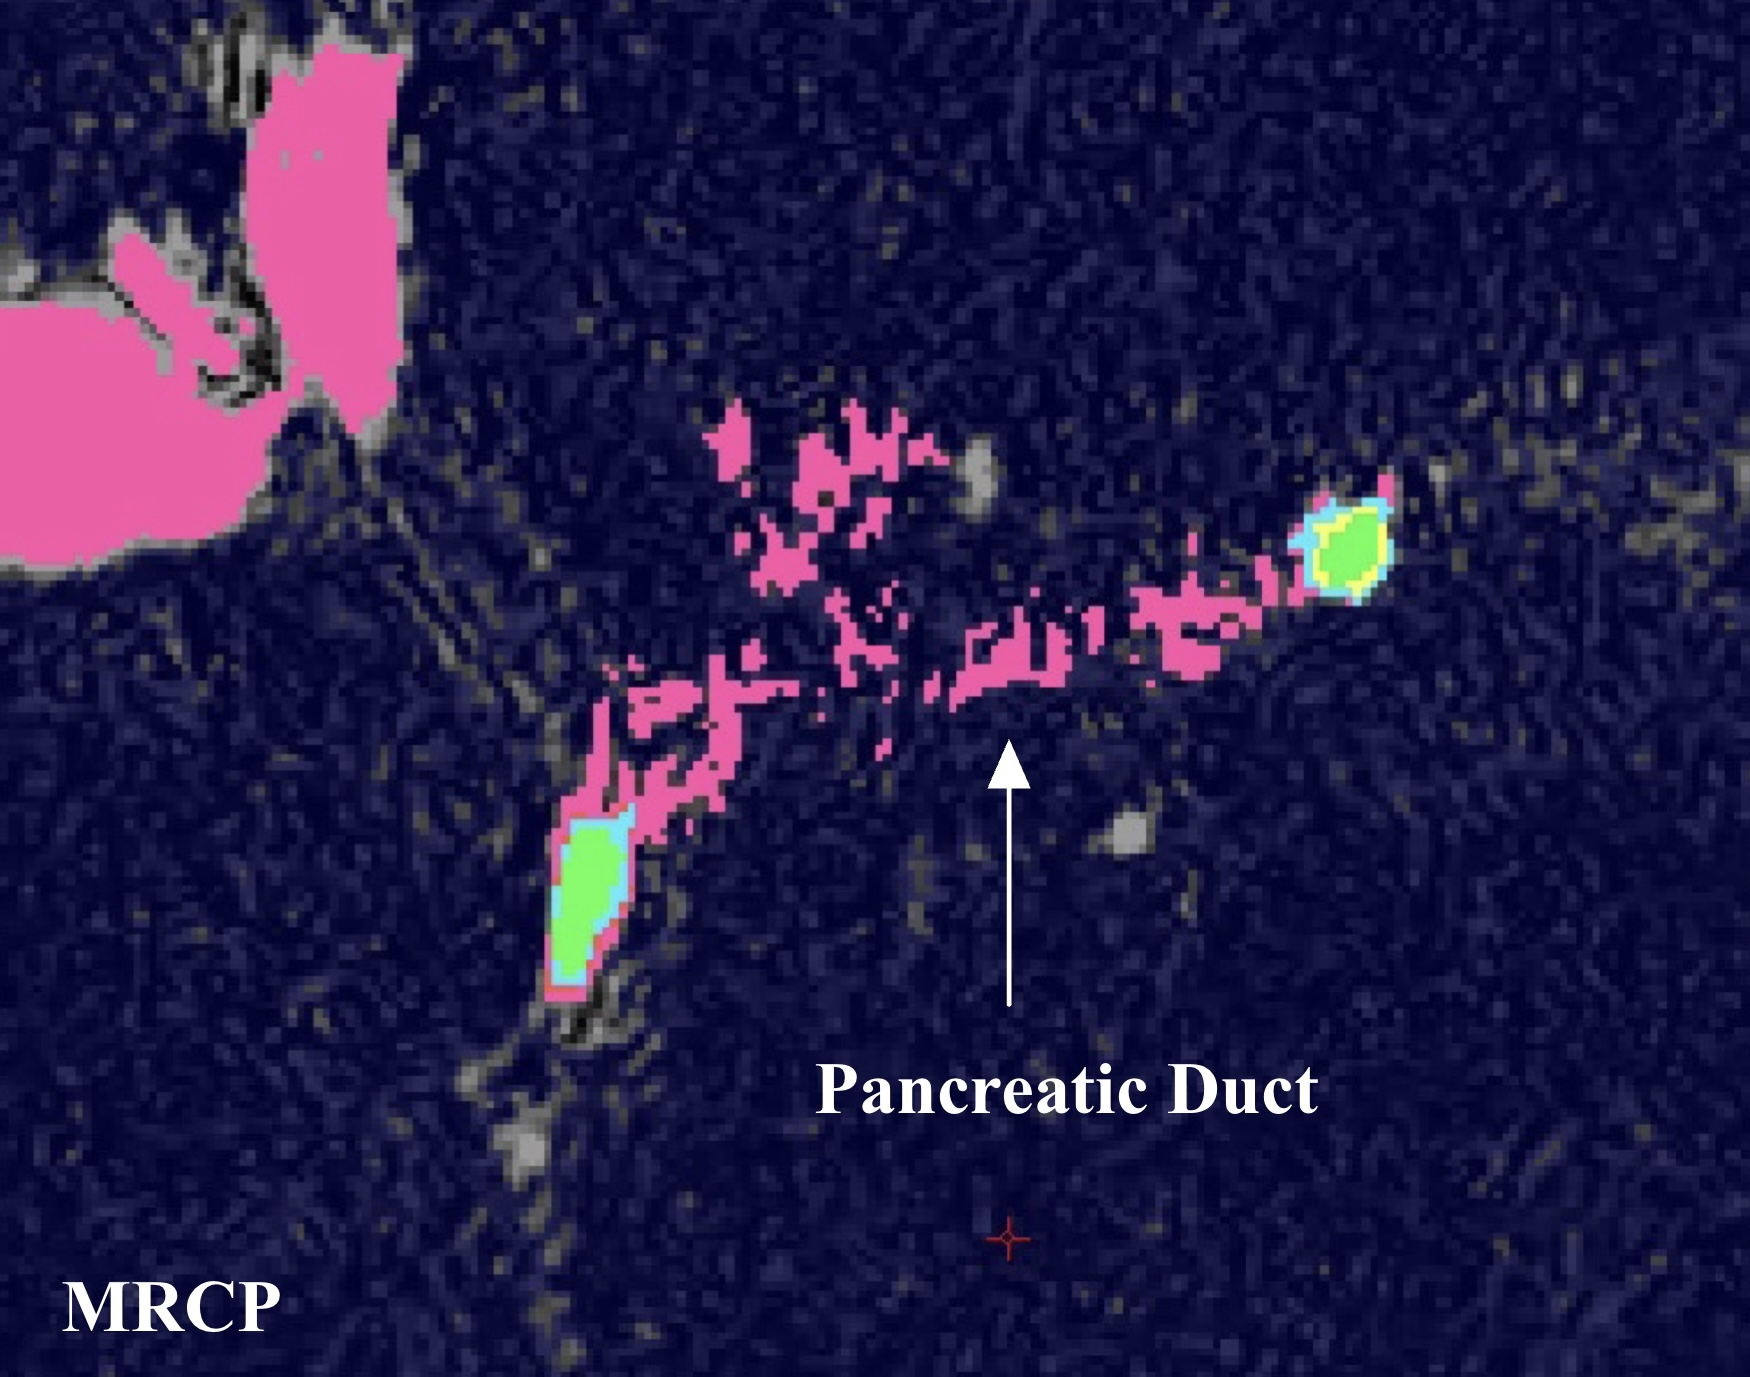
\includegraphics[width=\textwidth]{figures/MRCP.jpg}
                % \caption{\scriptsize{Total_Process}}
            \end{figure}
        \end{column}
    \end{columns}

    \vspace{0.05\textwidth}


    %  The simulation results are compared with the in-vivo measurements done in endoscopic retrograde cholangiopancreatography (ERCP), and the correlation between the ductal pressure drop and the patient pain score is analyzed.

    \begin{figure}[H]
        \centering
        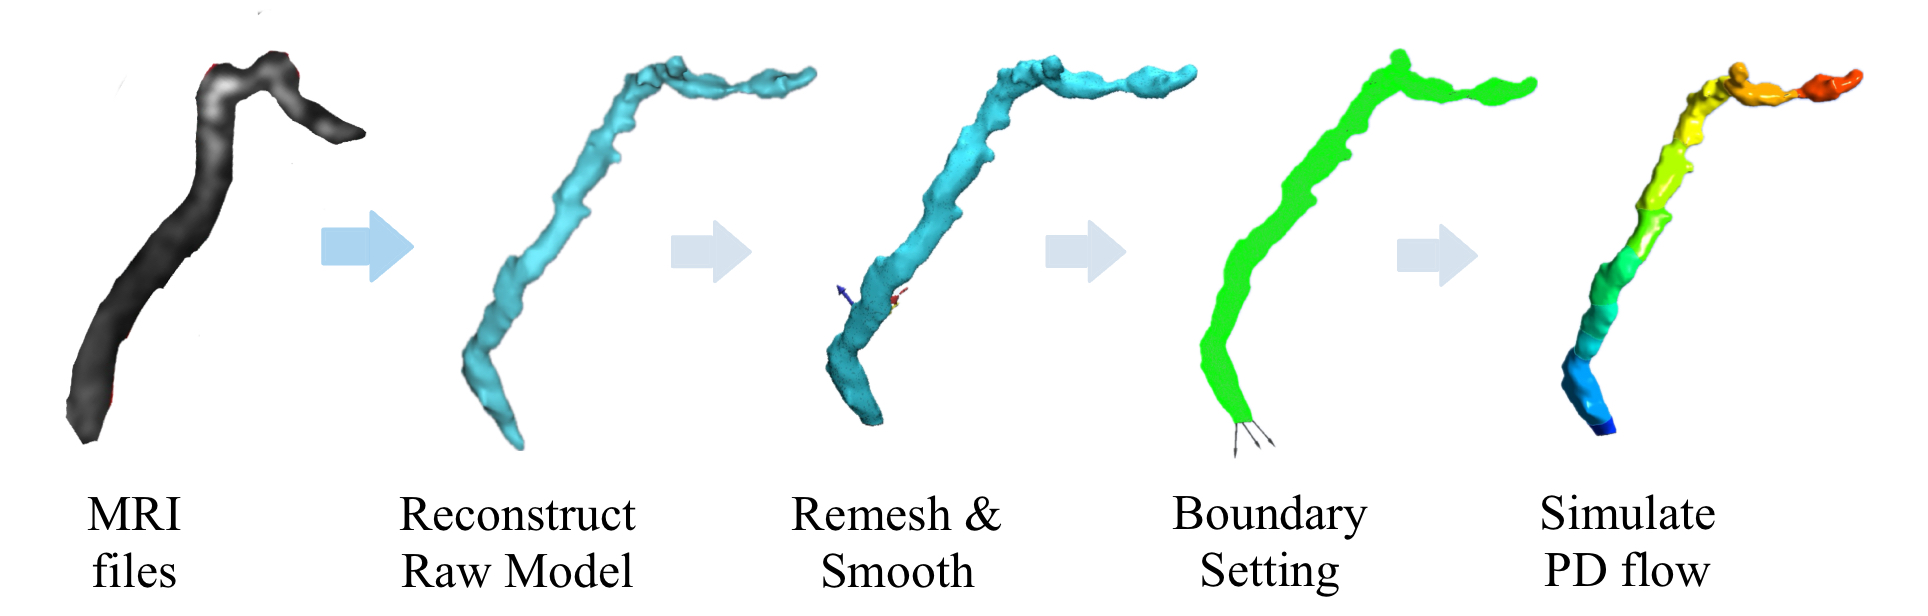
\includegraphics[width=\textwidth]{figures/Process-CFX_Total.jpg}
        % 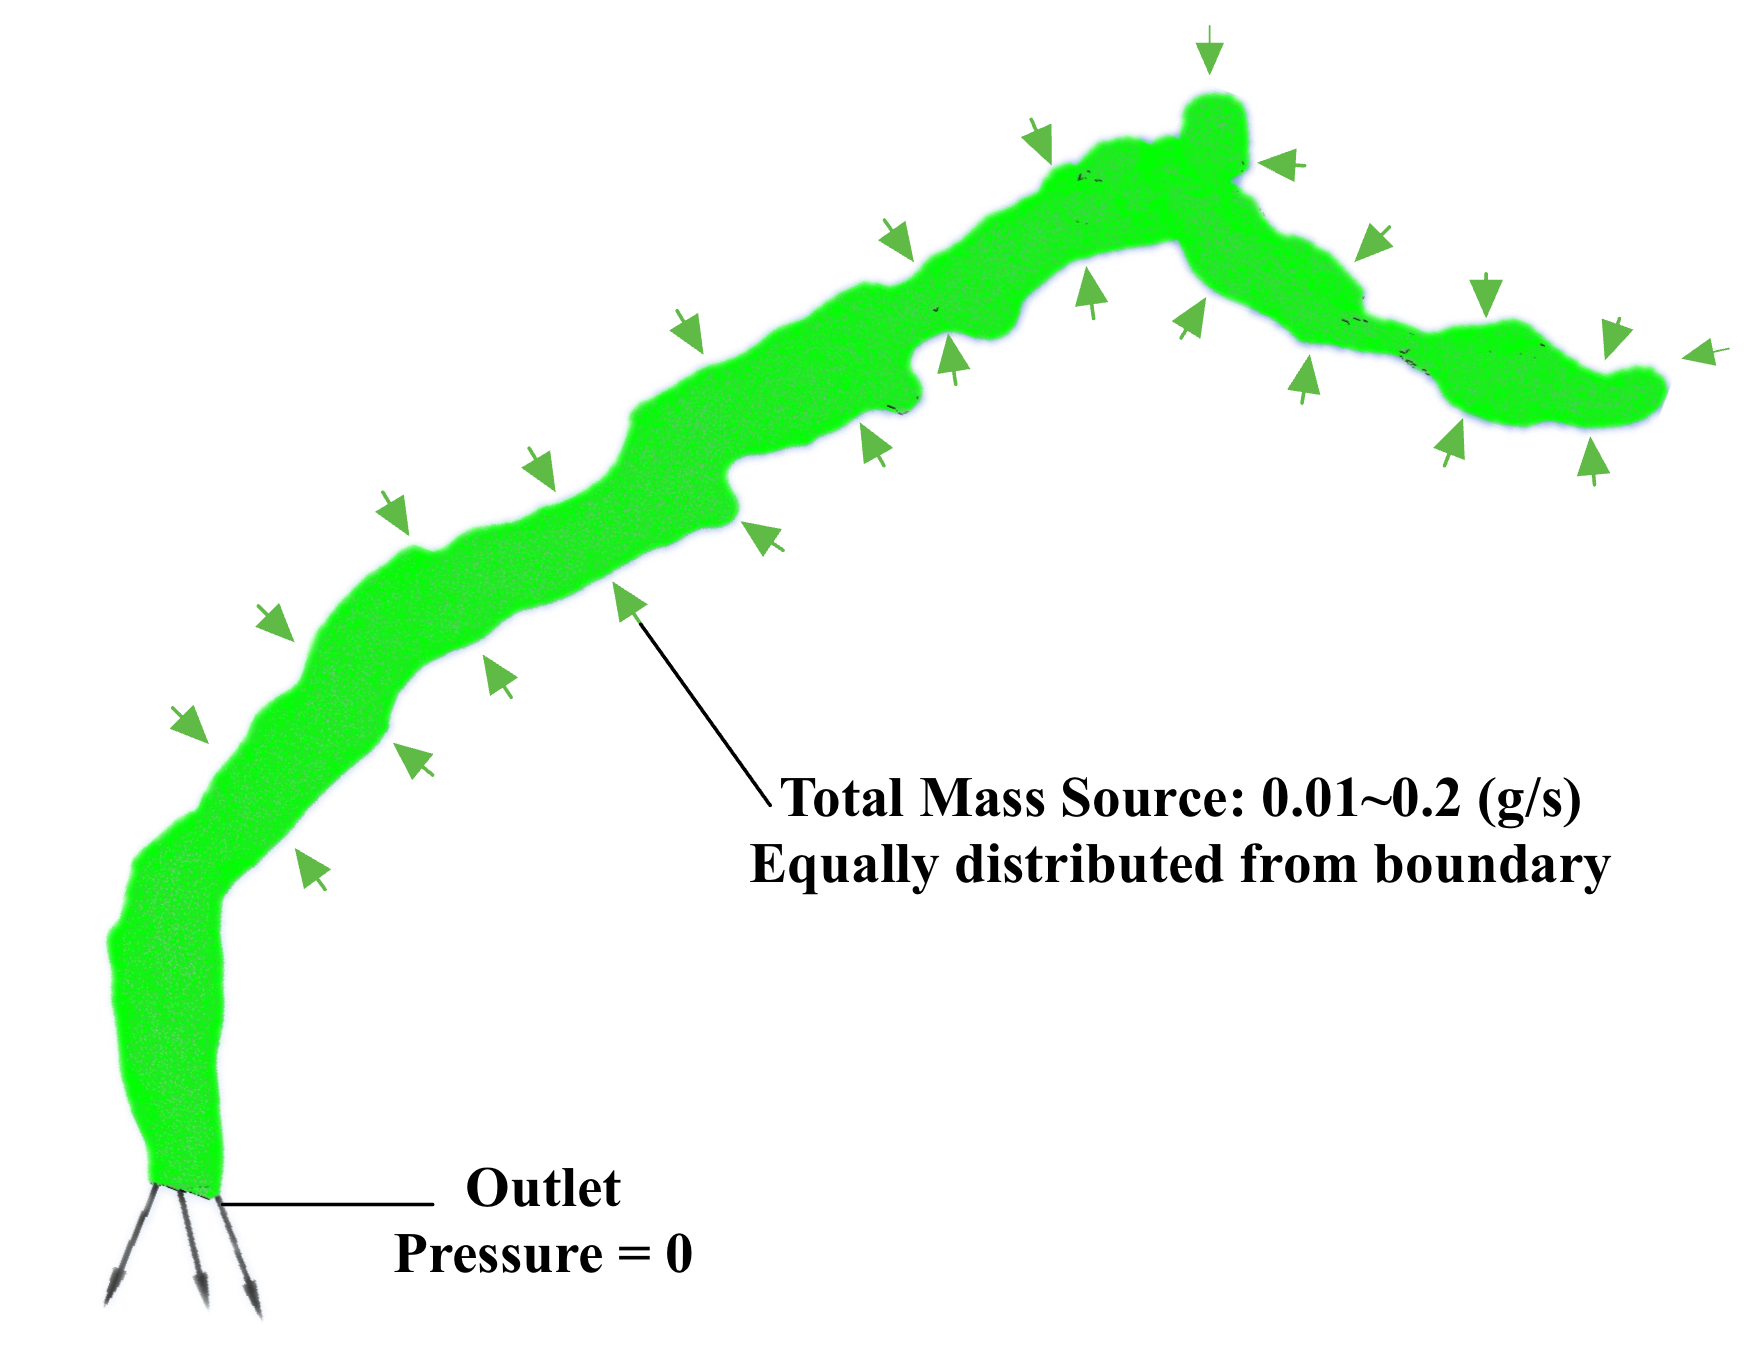
\includegraphics[width=0.3\textwidth]{figures/PD_BC.jpg}
        % \caption{\scriptsize{Total_Process}}
    \end{figure}

\end{frame}





% Page - Pipeline: From MRI to CFD Simulation (2)  %%%%%%%%%%%%%%%%%%%%%%%%%%%%%%%%%%%%%
\begin{frame}
    \fontsize{8pt}{10pt}\selectfont
    \frametitle{Pipeline: From MRI to CFD Simulation (2) }
    \vspace{0.02\textwidth}

    \begin{columns}
        \begin{column}{0.6\textwidth}
            In order to investigate the correlation between PD pressure and abdominal pain, 
            patient-specific image-based CFD analysis of PD flows has been performed.
            
            \vspace{0.02\textwidth}


            \begin{itemize}
                \item   3D model of the PD is reconstructed from: magnetic resonance cholangiopancreatography (MRCP)
                \item Simulation is performed to determine the flow pattern and measure the pressure drop across the duct.
            \end{itemize}

            
            
        \end{column}

        \begin{column}{0.45\textwidth}

            \begin{figure}[H]
                \centering
                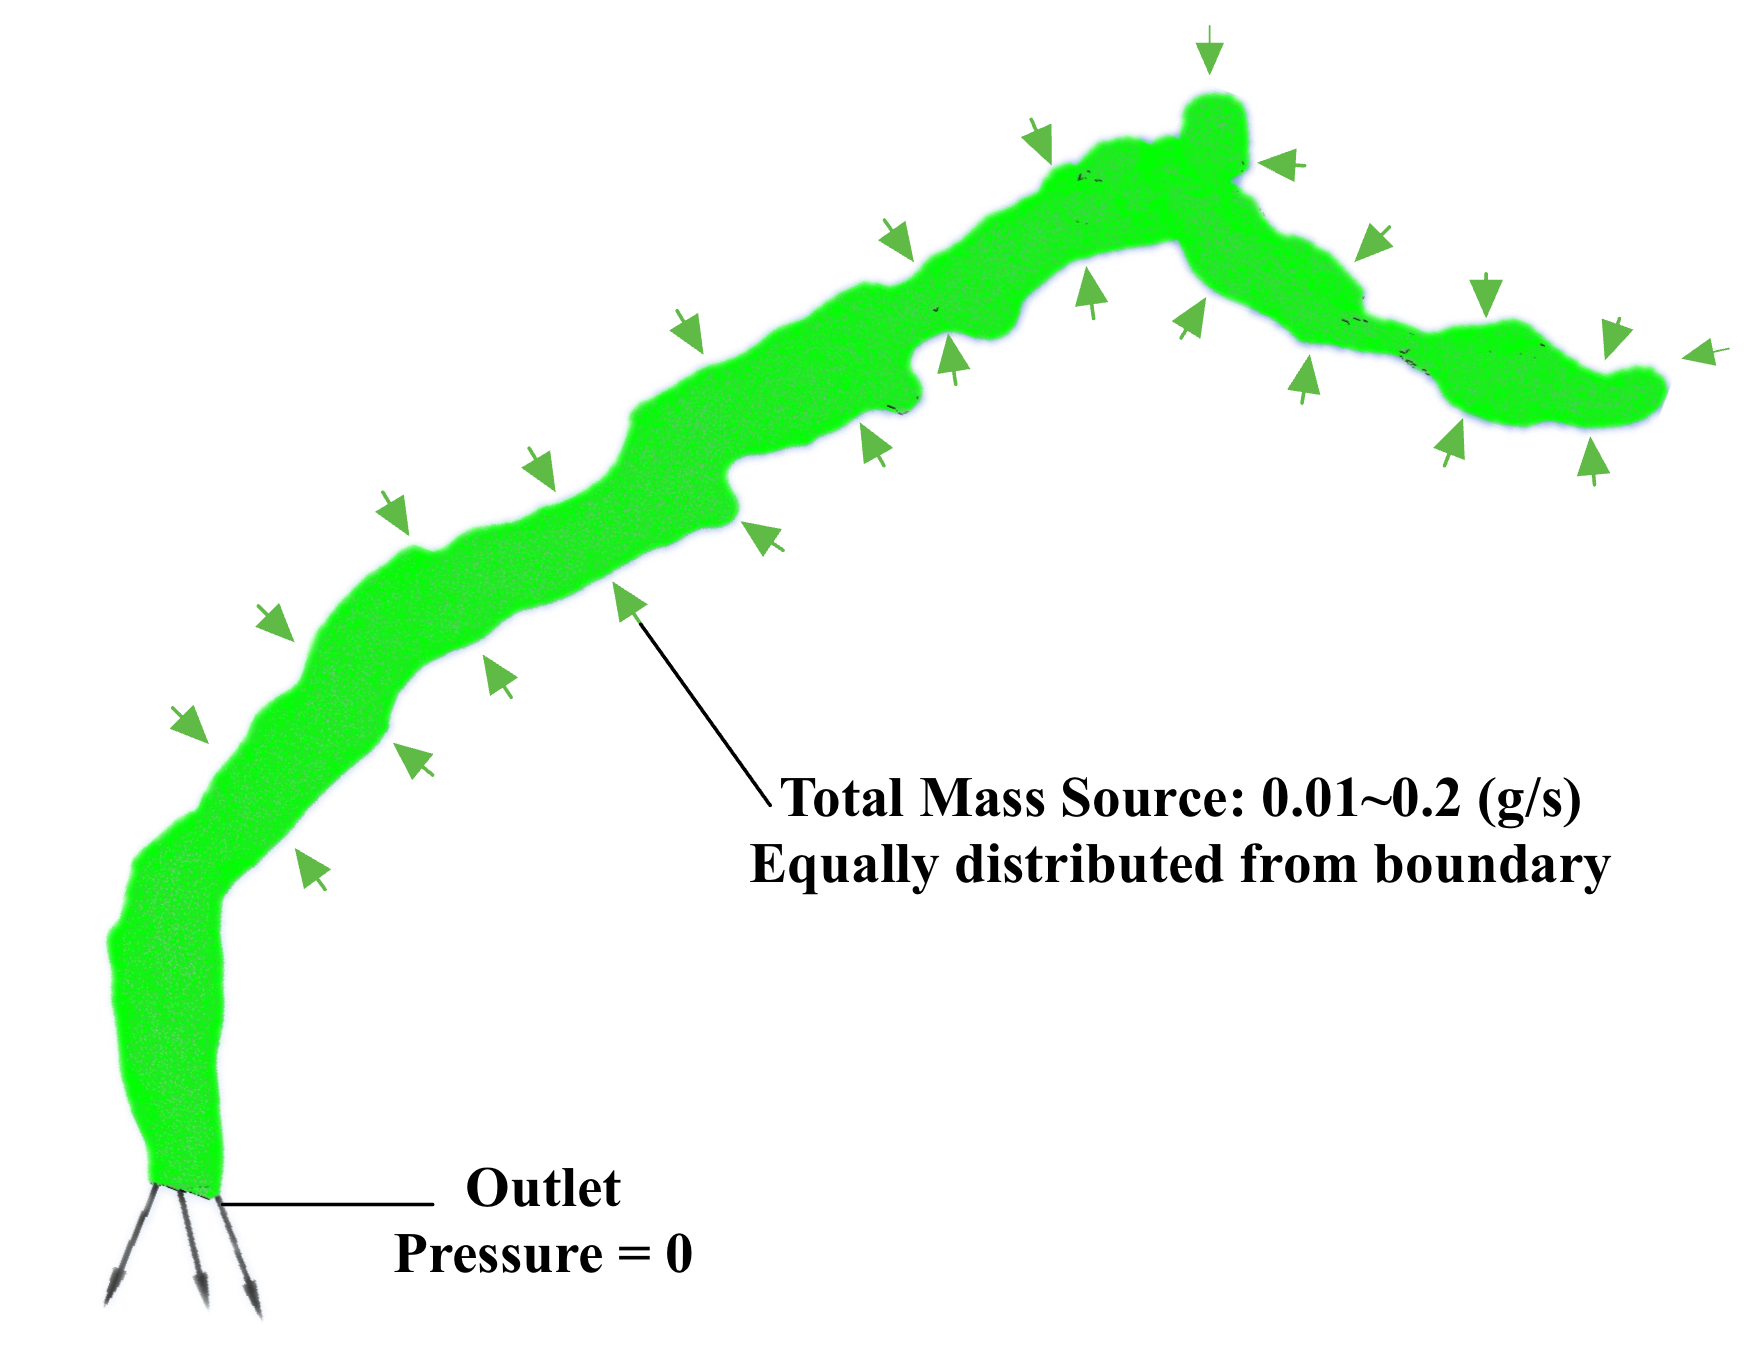
\includegraphics[width=\textwidth]{figures/PD_BC.jpg}
                % \caption{\scriptsize{Total_Process}}
            \end{figure}
        \end{column}
    \end{columns}

    % \vspace{0.05\textwidth}

    %  The simulation results are compared with the in-vivo measurements done in endoscopic retrograde cholangiopancreatography (ERCP), and the correlation between the ductal pressure drop and the patient pain score is analyzed.

    \begin{columns}
        \begin{column}{0.55\textwidth}
            \begin{figure}[H]
                \centering
                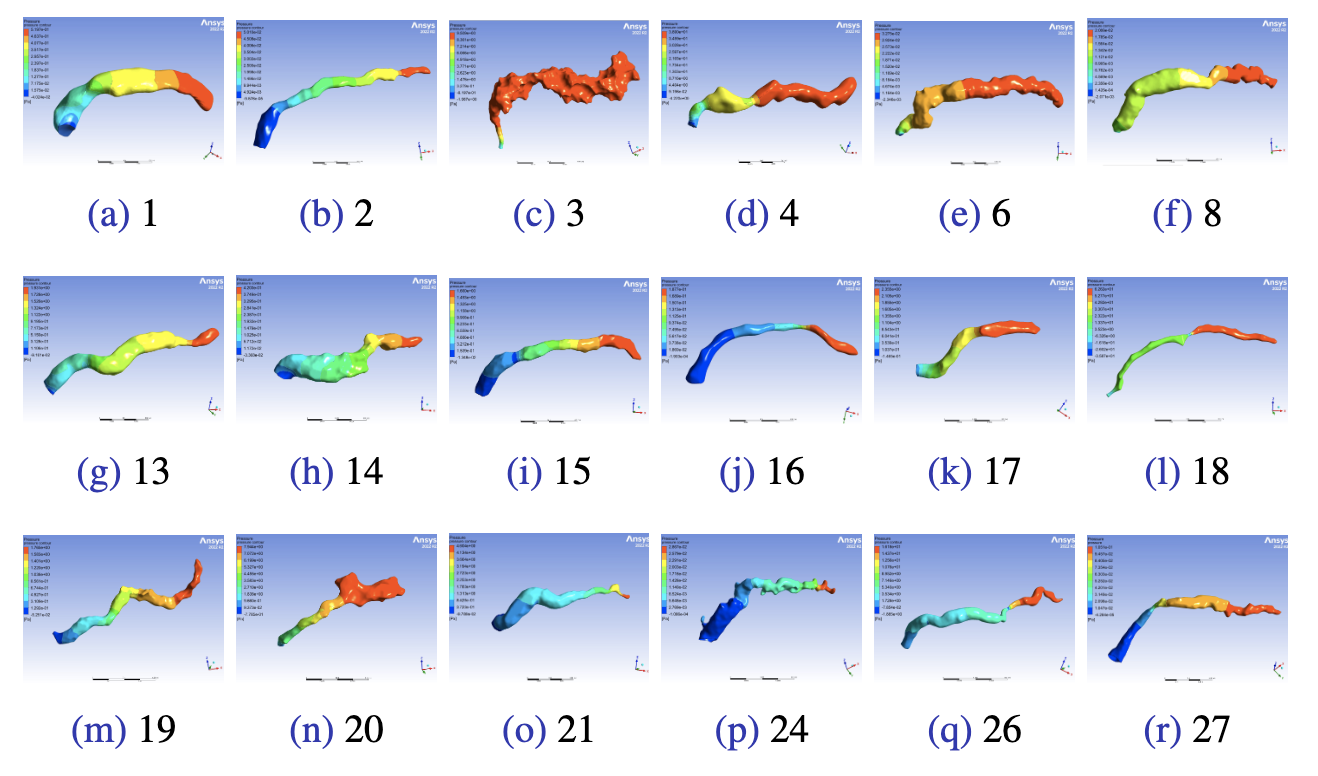
\includegraphics[width=\textwidth]{figures/Result_CFX.jpg}
                % 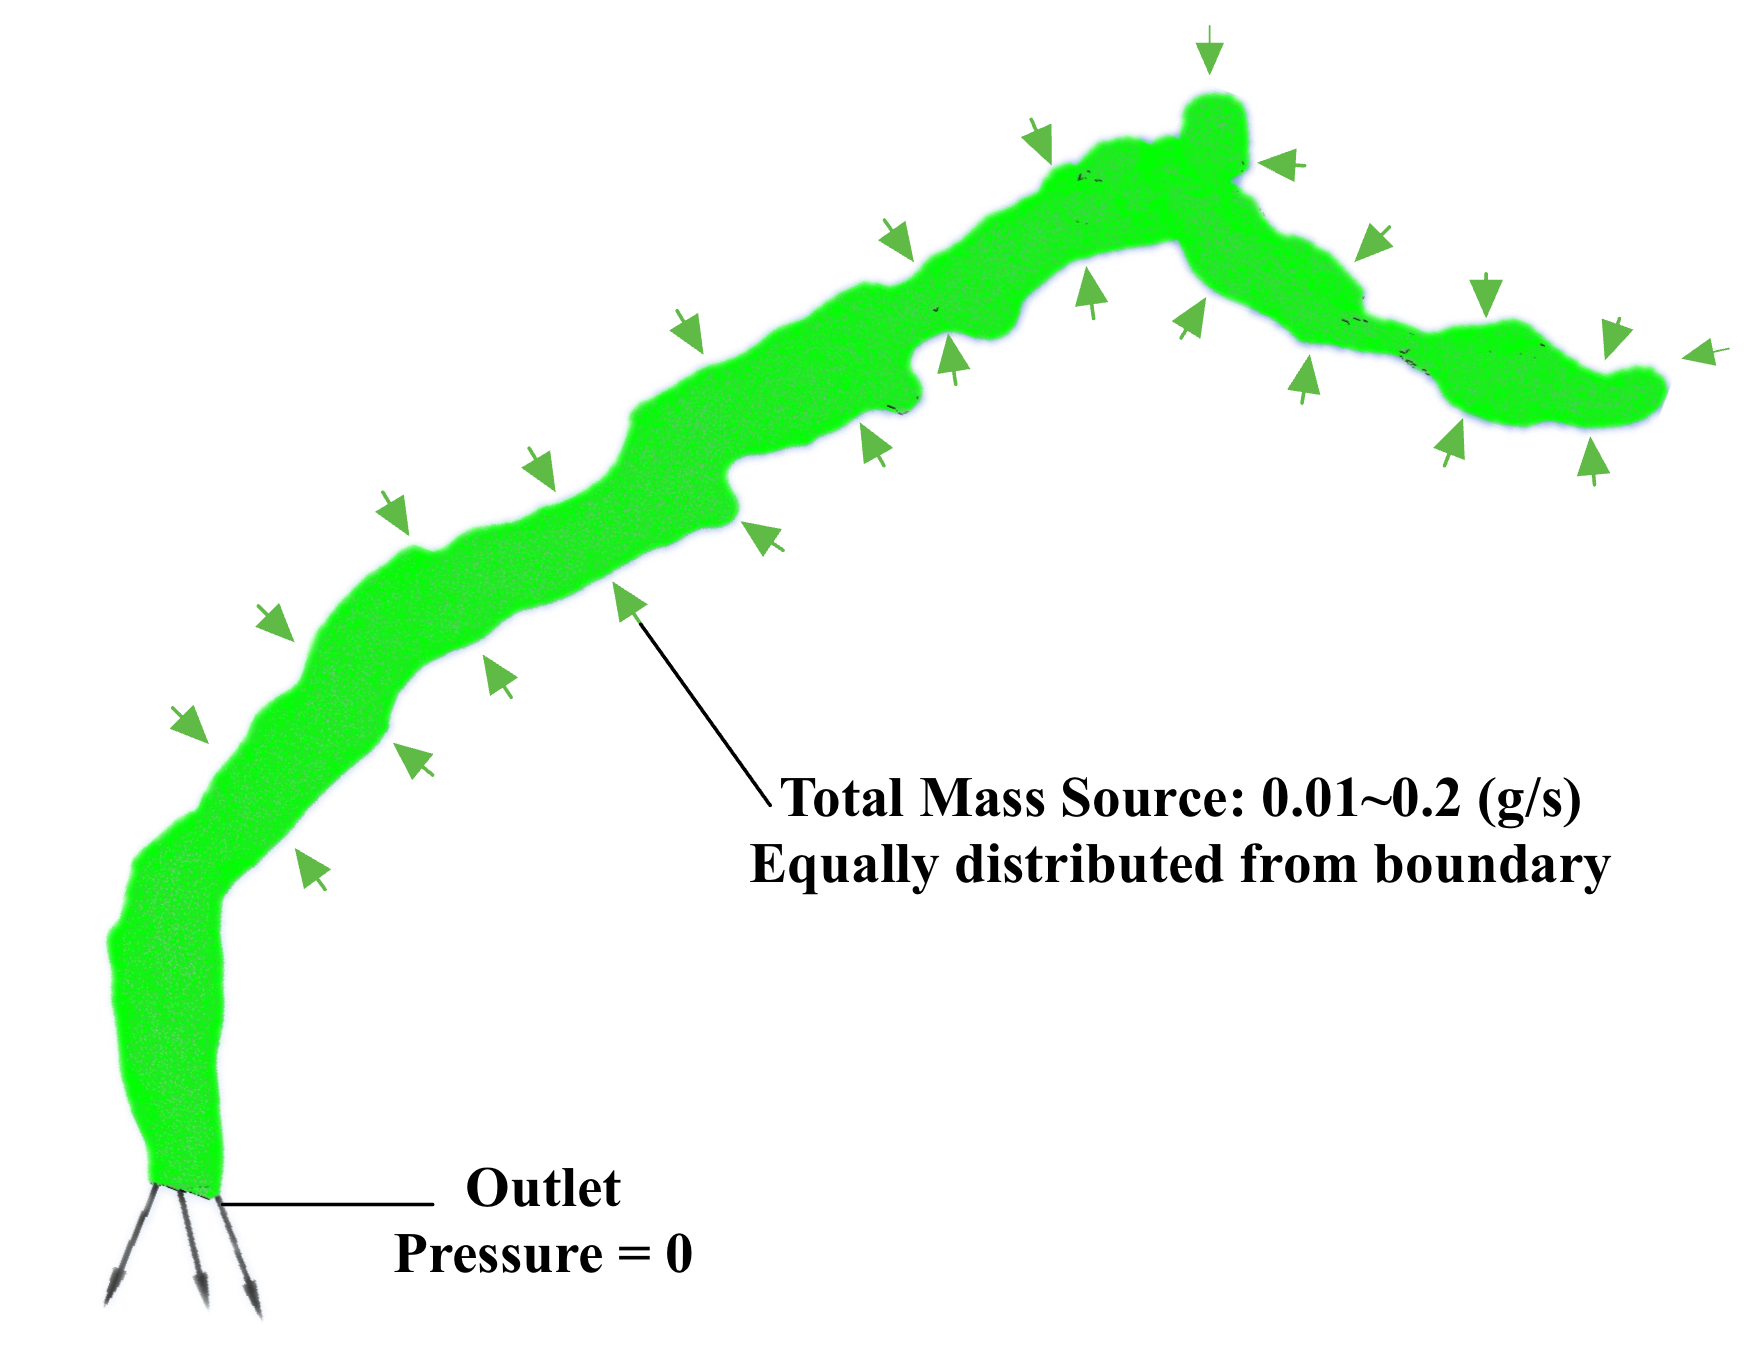
\includegraphics[width=0.3\textwidth]{figures/PD_BC.jpg}
                % \caption{\scriptsize{Total_Process}}
            \end{figure}


        \end{column}


        \begin{column}{0.45\textwidth}
            \begin{figure}[H]
                \centering
                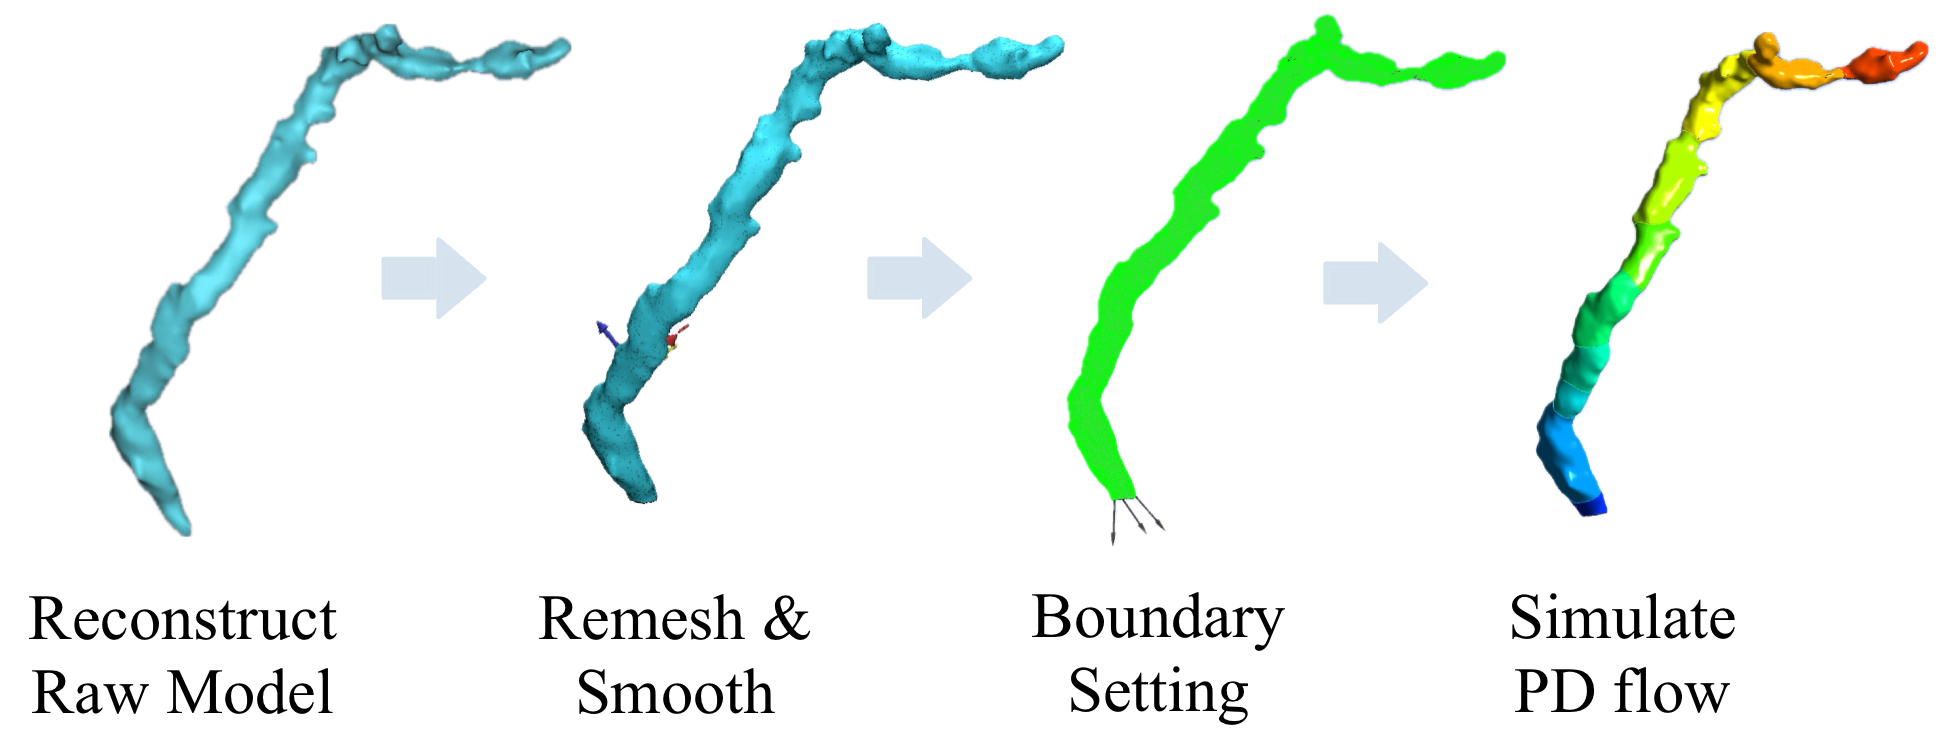
\includegraphics[width=1.1\textwidth]{figures/Process-CFX.jpg}
                % 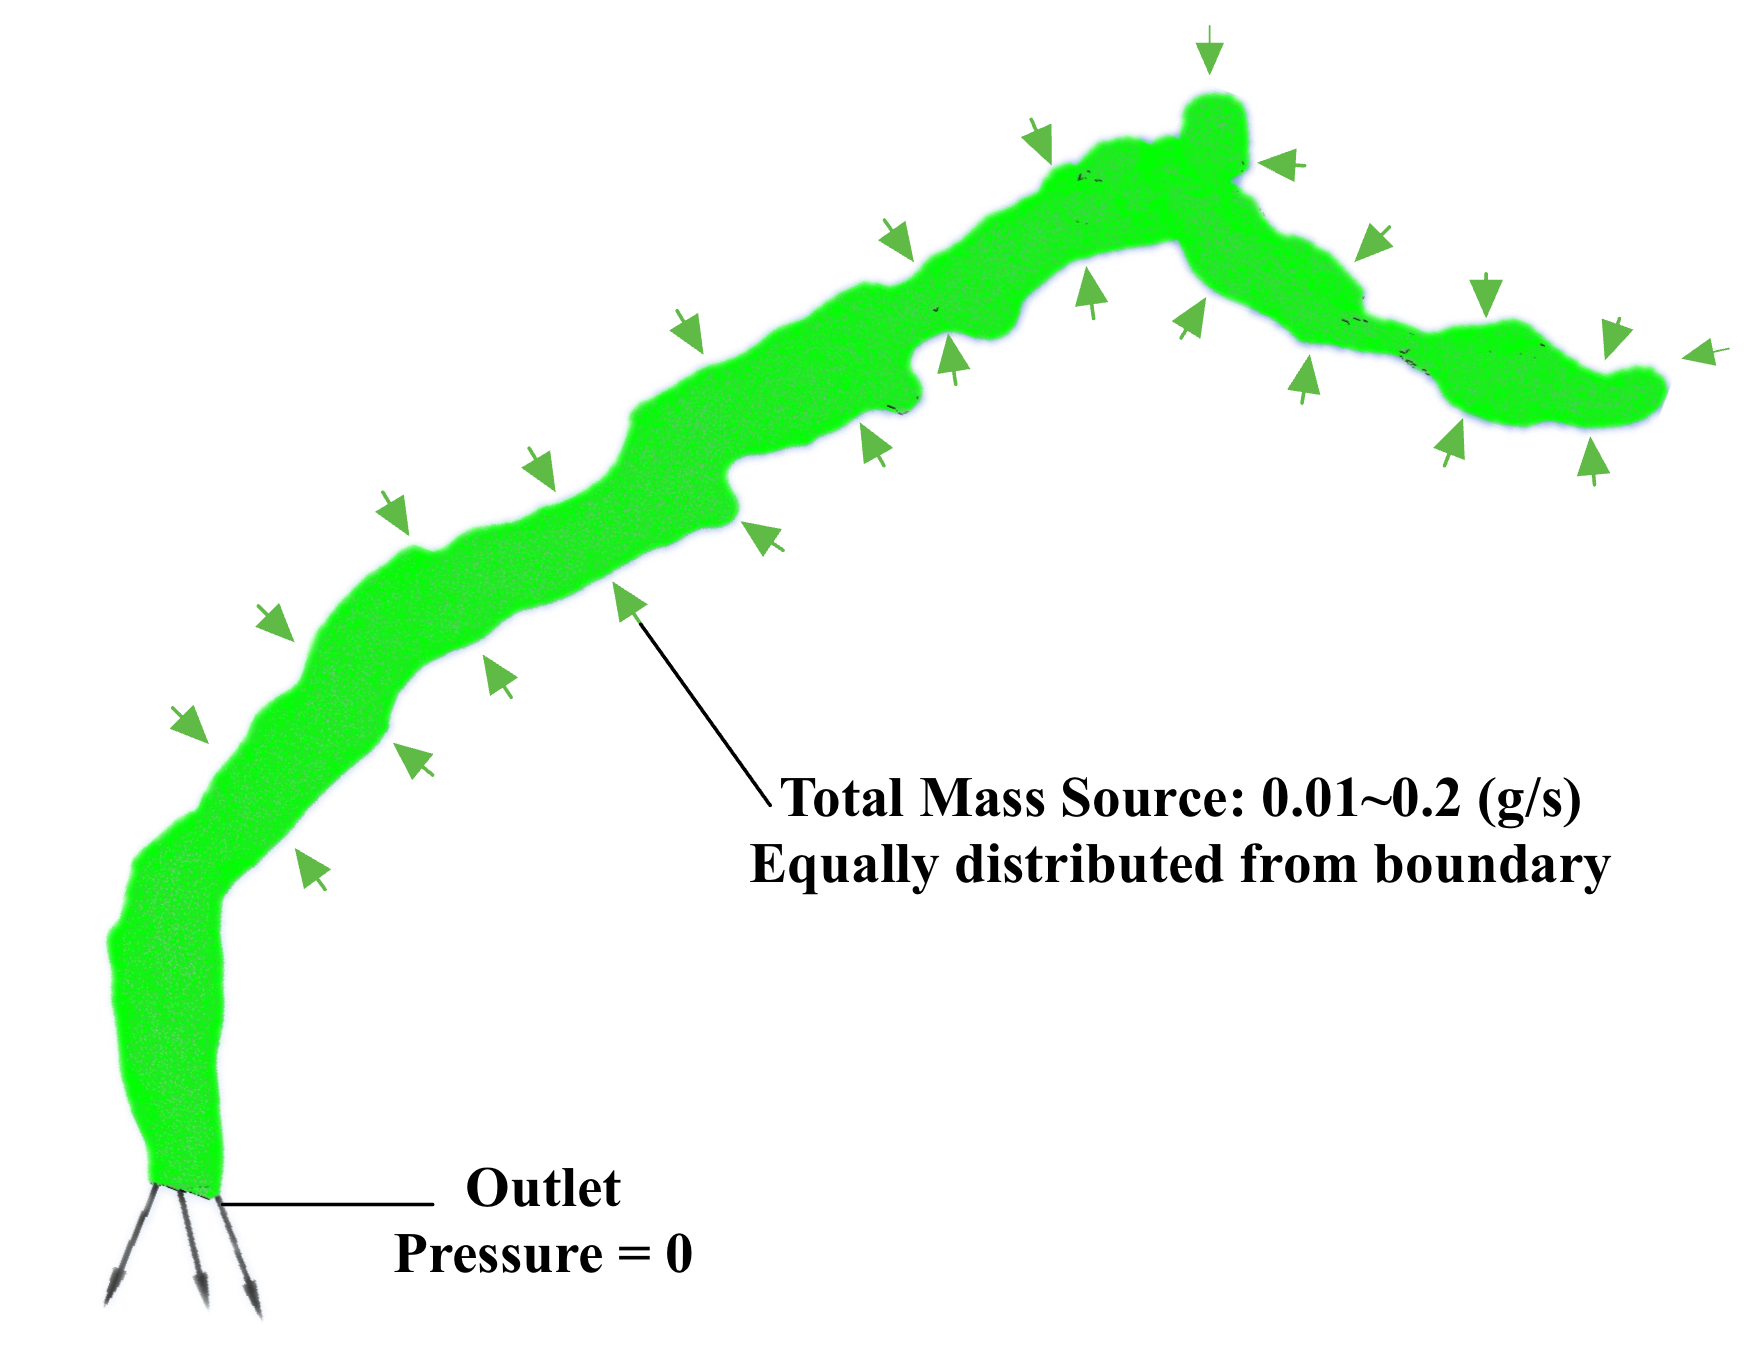
\includegraphics[width=0.3\textwidth]{figures/PD_BC.jpg}
                % \caption{\scriptsize{Total_Process}}
            \end{figure}



        \end{column}
        
    \end{columns}
    

\end{frame}













% Page - Result: Compare Wirh Clinical Data  %%%%%%%%%%%%%%%%%%%%%%%%%%%%%%%%%%%%%
\begin{frame}
    \fontsize{8pt}{10pt}\selectfont
    \frametitle{Result: Compare Wirh Clinical Data }
    
    Correlation of ERCP Pressure Drop (clinical data) and CFD Pressure Drop ($R^2=0.95$):
    
    \vspace{-0.015\textwidth}

    \begin{columns}
        \begin{column}{0.4\textwidth}

            \begin{table}[h!]
                \centering
                \renewcommand{\arraystretch}{1.2} % Adjust row height for better readability
                \setlength{\tabcolsep}{12pt} % Adjust column separation for better spacing
                \resizebox{\textwidth}{!}{
                \begin{tabular}{l c c }
                \hline
                \textbf{Q}         & \textbf{Tail-Head} & \textbf{0.1} \\ \hline
                \textbf{1}         & 1                  & 0.0488       \\ 
                \textbf{2}         & 2                  & 0.55         \\ 
                \textbf{4}         & 4                  & 2.21         \\ 
                \textbf{6}         & 6                  & 0.317        \\ 
                \textbf{8}         & 8                  & 0.117        \\ \hline
                \end{tabular}
                }
                \label{tab:transposed_table_sci}
                \end{table}
                
                
                \vspace{-0.05\textwidth}


                
        \end{column}

        \begin{column}{0.5\textwidth}

            \begin{figure}[H]
                \centering
                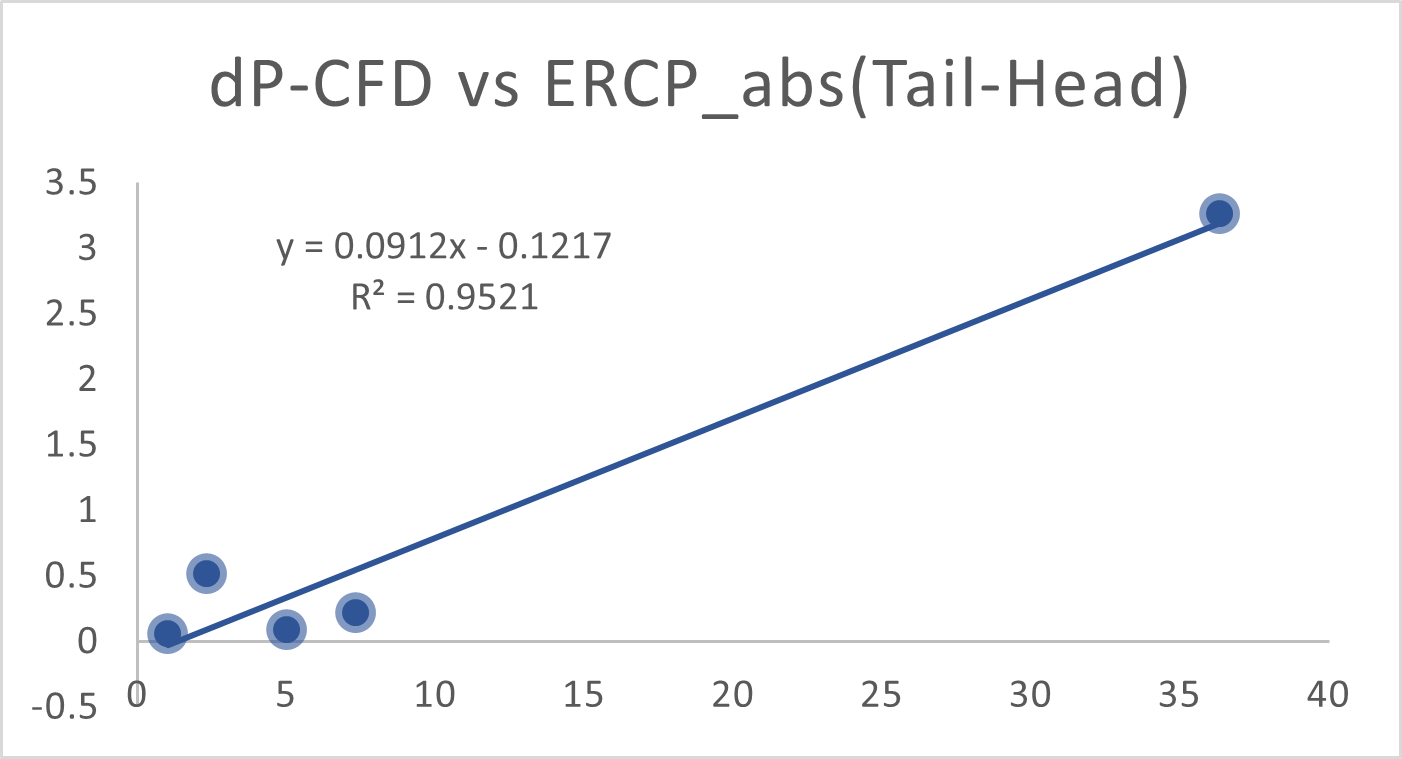
\includegraphics[width=\textwidth]{figures/Result_ERCP.png}
            \end{figure}
        \end{column}
    \end{columns}

    \vspace{0.02\textwidth}


    Correlation of Pre-Post Pain Score (clinical data) and CFD Pressure Drop ($R^2=0.61$):

    \vspace{-0.03\textwidth}





    \begin{columns}
        \begin{column}{0.4\textwidth}

            \begin{table}[h!]
                \centering
                \renewcommand{\arraystretch}{1.3} % Adjust row height for better readability
                \setlength{\tabcolsep}{10pt} % Adjust column separation for better spacing
                
                \resizebox{\textwidth}{!}{
                \begin{tabular}{l c c }
                \hline
                \textbf{ID} & \textbf{Pain Score} & \textbf{$dP_{cfd}$ ($\dot{M}=0.1\,g/s$)} \\ \hline
                \textbf{2}       & 8                              & 1.05                                  \\ 
                \textbf{6}       & 4                              & 1.355                                 \\ 
                \textbf{45}      & 2                              & 0.234                                 \\ 
                \textbf{50}      & 2                              & 0.163                                 \\ 
                \textbf{58}      & 3                              & 0.789                                 \\ 
                \textbf{61}      & 8                              & 1.25                                  \\ 
                \textbf{69}      & 1                              & 0.077                                 \\ 
                \textbf{70}      & 3                              & 0.219                                 \\ \hline
                \end{tabular}
                }
                \tiny
                \label{tab:comparison_transposed}
                \end{table}

                \vspace{-0.05\textwidth}



                
        \end{column}

        \begin{column}{0.5\textwidth}

            \begin{figure}[H]
                \centering
                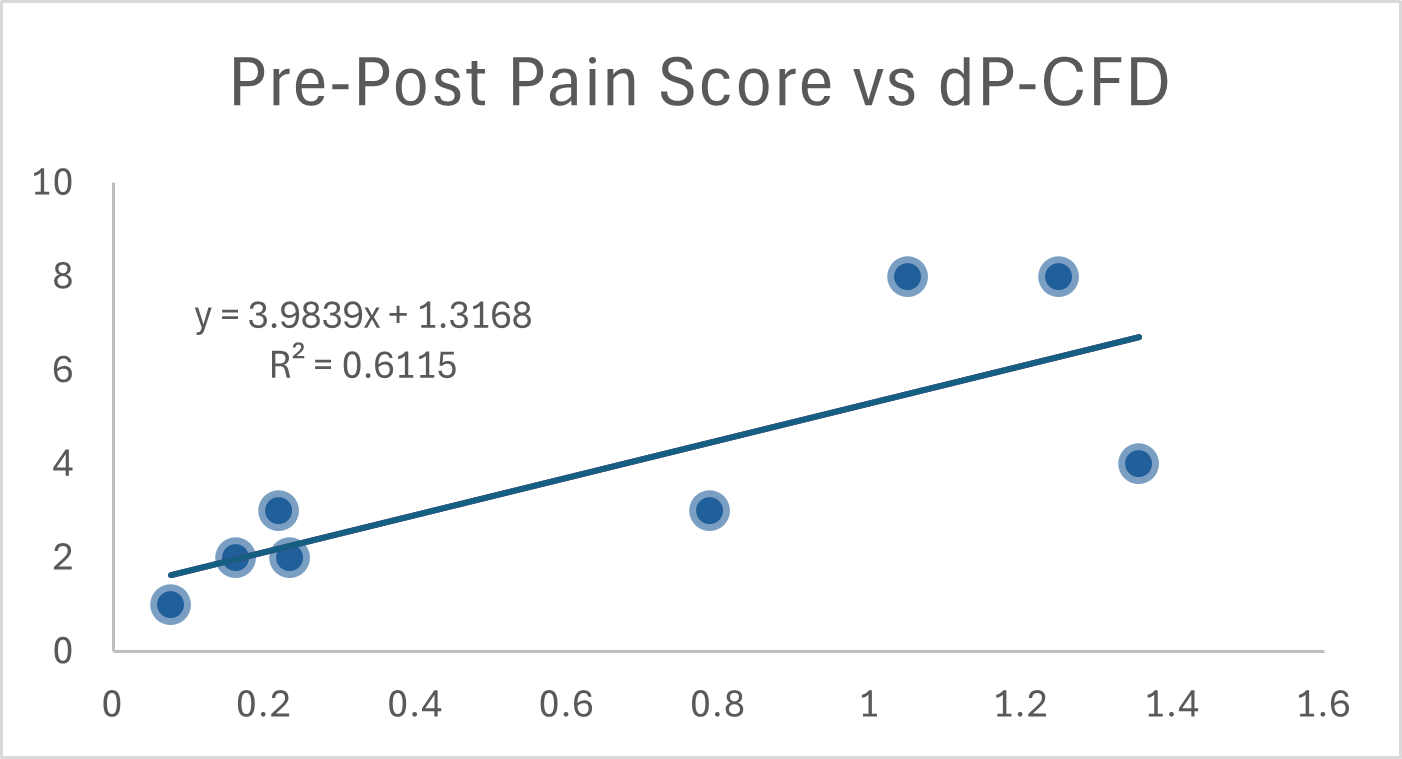
\includegraphics[width=\textwidth]{figures/Result_Painscore.jpg}
            \end{figure}
        \end{column}

    \end{columns}

    Now we have build up \textbf{patient-specific pipeline} 
    for Pressure measurement, compared to ERCP and 
    Pain score in limited cases, we have verified 
    the \textbf{effectiveness} of CFD pressure prediction
    based on MRI.

\end{frame}



% Page - Analytical Approach: Road Map For Pressure Prediction %%%%%%%%%%%%%%%%%%%%%%%%%%%%%%%%%%%%%
\begin{frame}
    \fontsize{8pt}{10pt}\selectfont
    \frametitle{Analytical Approach: Road Map For Pressure Prediction }
    
    However, CFD simulation require high-computational
    resources, 


        
    \begin{figure}[H]
        \centering
        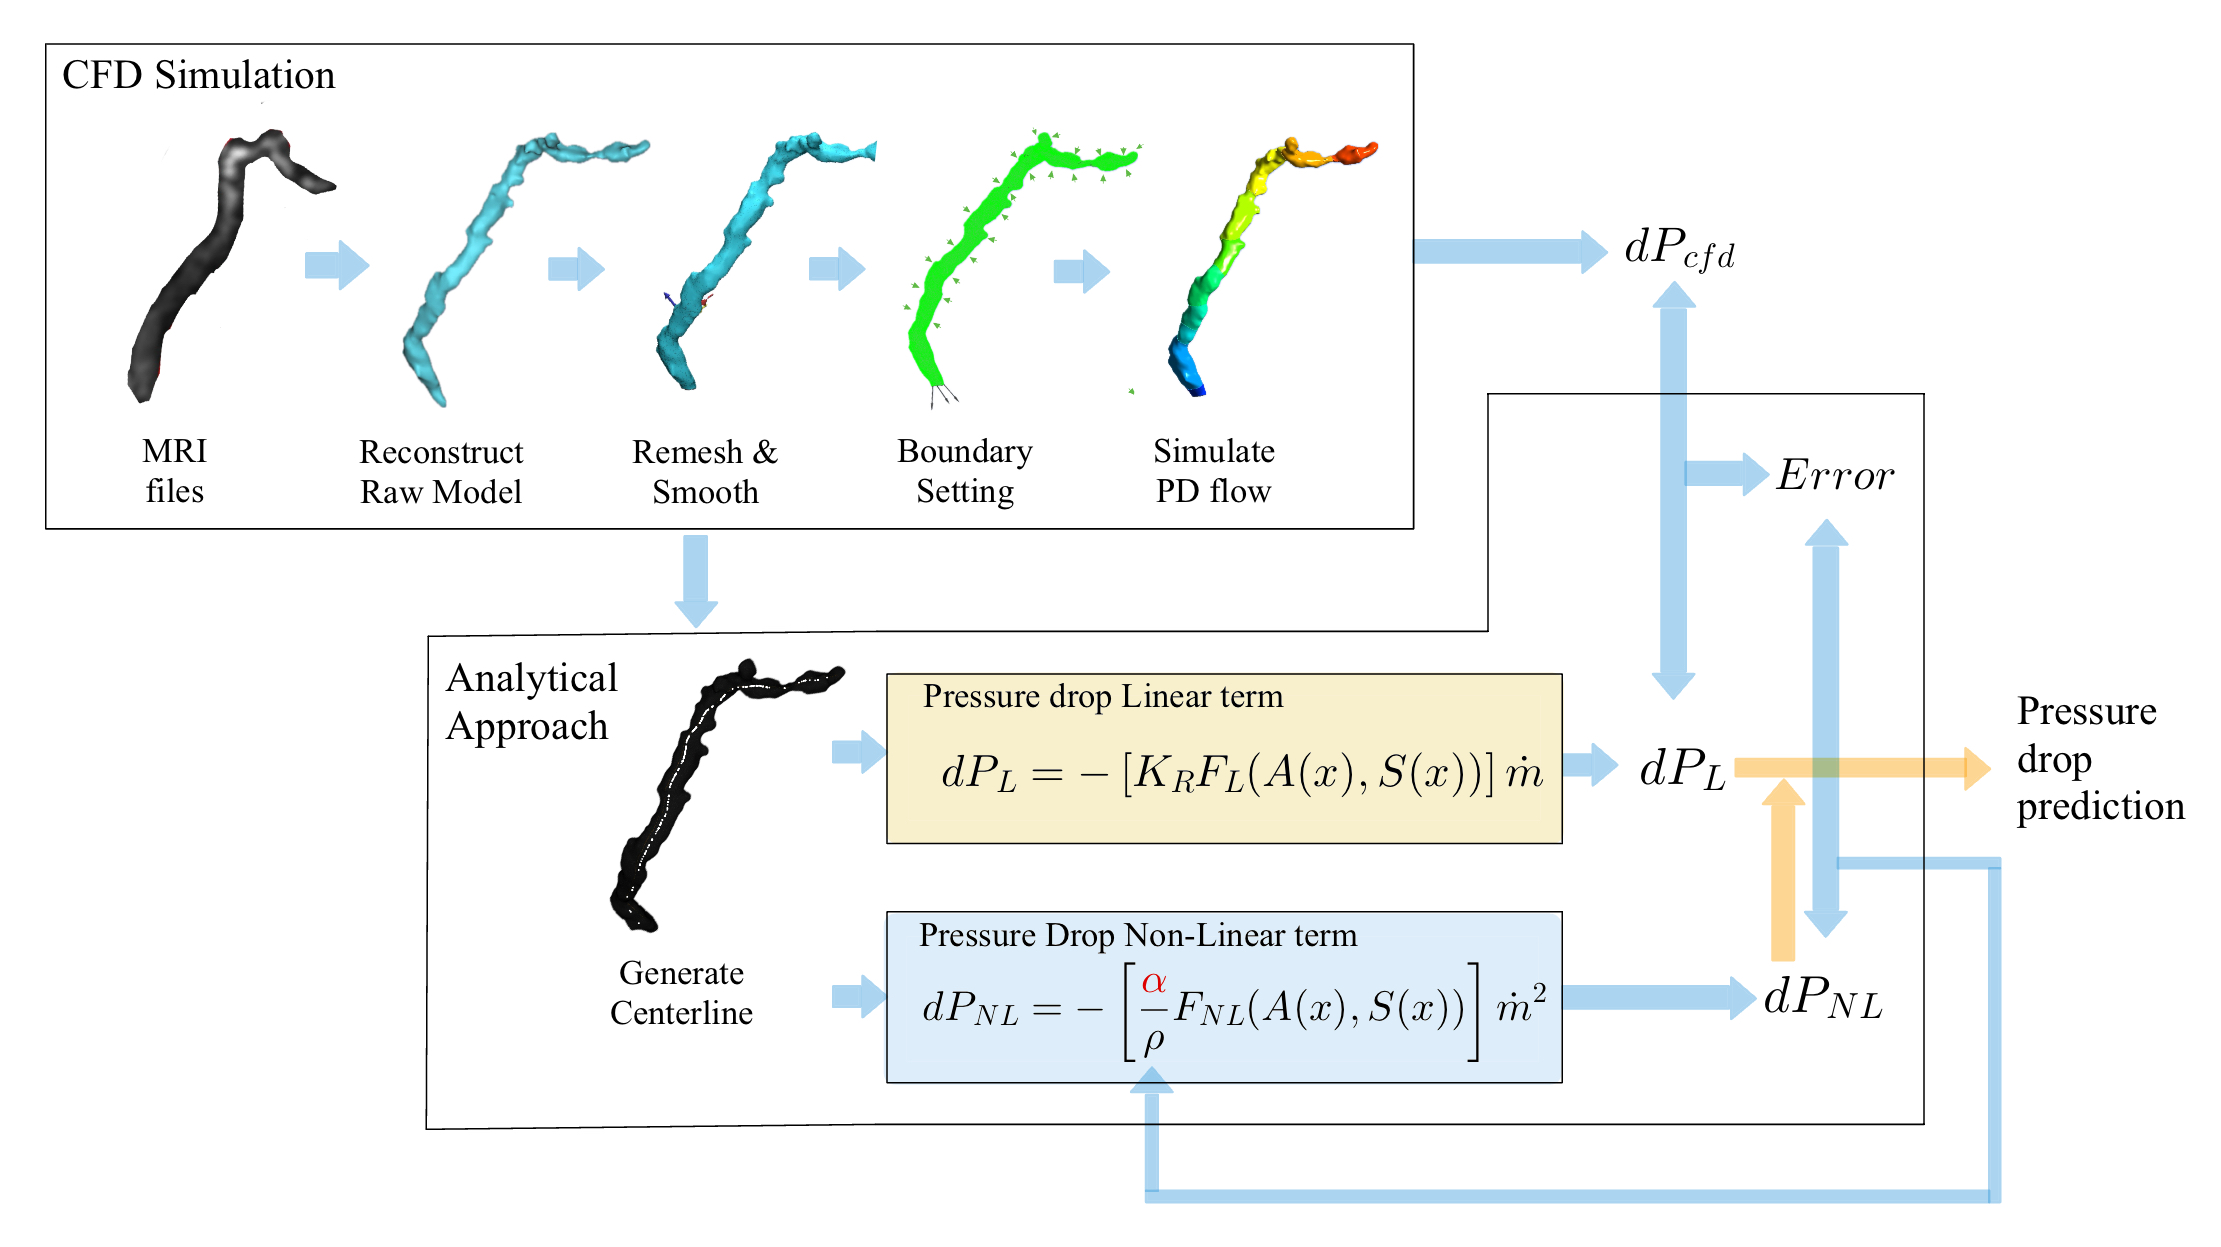
\includegraphics[width=\textwidth]{figures/Process-Total.jpg}
        % \caption{Road map for pressure prediction}
    \end{figure}

    So we developed analytical approach 
    using CFD and ERCP result for limited cases,


    and applying machine learning algorithm to performe
    pressure prediction in clinical environment.
    

    

\end{frame}







% Page - Analytical Approach  %%%%%%%%%%%%%%%%%%%%%%%%%%%%%%%%%%%%%
\begin{frame}
    \fontsize{8pt}{10pt}\selectfont
    \frametitle{Analytical Approach }


    Formula:

    \begin{columns}
        \begin{column}{0.6\textwidth}
            \begin{equation*}
                \left\{
                \begin{aligned}
                & \frac{\partial A}{\partial t} + \frac{\partial Q}{\partial x} = V_{gm} \\
                & \frac{\partial Q}{\partial t} + \frac{\partial}{\partial x} \left( \alpha \frac{Q^2}{A} \right) + \frac{A}{\rho} \frac{\partial P}{\partial x} + K_R \frac{Q}{A} = 0
                \end{aligned}
                \right.
                \Rightarrow
            \end{equation*}
            
        \end{column}
        \begin{column}{0.5\textwidth}
            \begin{equation*}
            \left\{
            \begin{aligned}
            & \quad \rho Q = \int_{x} \Delta \dot{M} dx\\
            & \quad P = - \int_{x} [K_R \frac{\rho Q}{A^2} + \frac{\rho}{A}\frac{\partial}{\partial x}(\alpha\frac{Q^2}{A})] dx
            \end{aligned}
            \right.
            \end{equation*}
            
        \end{column}
    \end{columns}

    We could separate calculate the linear and non-linear part:


            {\tiny
            \begin{equation}
                P = -k_R \textcolor{red}{\dot{m}}
                \left[
                \int_{x_0}^{x_{max}}
                \frac{1}{A^2} 
                \left(
                \int_{x_0}^x
                dS 
                \right) 
                dx 
                \right]
                 - \frac{\alpha}{\rho}  \textcolor{red}{{\dot{m}^2}}
                \left[  
                \int_{x_0}^{x_{max}} 
                \frac{2}{A^2}  \Delta S(x)
                \left(
                \int_{x_0}^x
                dS
                \right) 
                dx 
                -  
                \int_{x_0}^{x_{max}}
                \frac{1}{A^3}
                \left(
                \int_{x_0}^x
                dS
                \right) ^2
                \frac{dA}{dx} 
                dx
                \right]
                \end{equation}
            }      
                
                \begin{itemize}
                    \item $K_R$ is resistance parameter.\\
                     Consider Poiseuille flow, $K_R = 8\pi \nu= 8\pi \frac{\mu}{\rho}$. For water, $\mu = 8.9 \times 10^{-4}$ (Pa $\cdot$ s)
                    \item $\dot{M}_T$ (kg/s) is the \textbf{total mass source}, 
                    means the total mass flow in rate of surface.
                    \item $S_T$ ($m^2$) is the total surface area of the duct
                    \item $\dot{m}$ $(kg/(s \cdot m^2))$ is $\frac{\dot{M}_T}{S_T}$, which is the mass source per unit area
                    \item $\Delta S(x)$ ($m^2$) is the round surface area for each segment of the centerline.
                    \item $A(x)$ ($m^2$) is the cross-sectional area of the duct
                \end{itemize}
                
                
                \begin{equation}
                    P = 
                    - [\frac{\textcolor{red}{\alpha}}{\rho} F_{NL}(A(x), S(x))] \dot{m} ^2 
                    - [K_R F_{L}(A(x), S(x))] \dot{m}
                \end{equation}
                
                In this equation, as we could obtain A(x), S(x) as pancreatic duct shape parameters, we could obtain the coefficient of $\dot{m}$ for each duct.
                

\end{frame}







% Page - Analytical Approach: Compare with CFD Data  %%%%%%%%%%%%%%%%%%%%%%%%%%%%%%%%%%%%%
\begin{frame}
    \fontsize{8pt}{10pt}\selectfont
    \frametitle{Analytical Approach: Compare with CFD Data }
    

    

    


    \begin{columns}
        \begin{column}{0.5\textwidth}

            \begin{figure}[H]
                \centering
                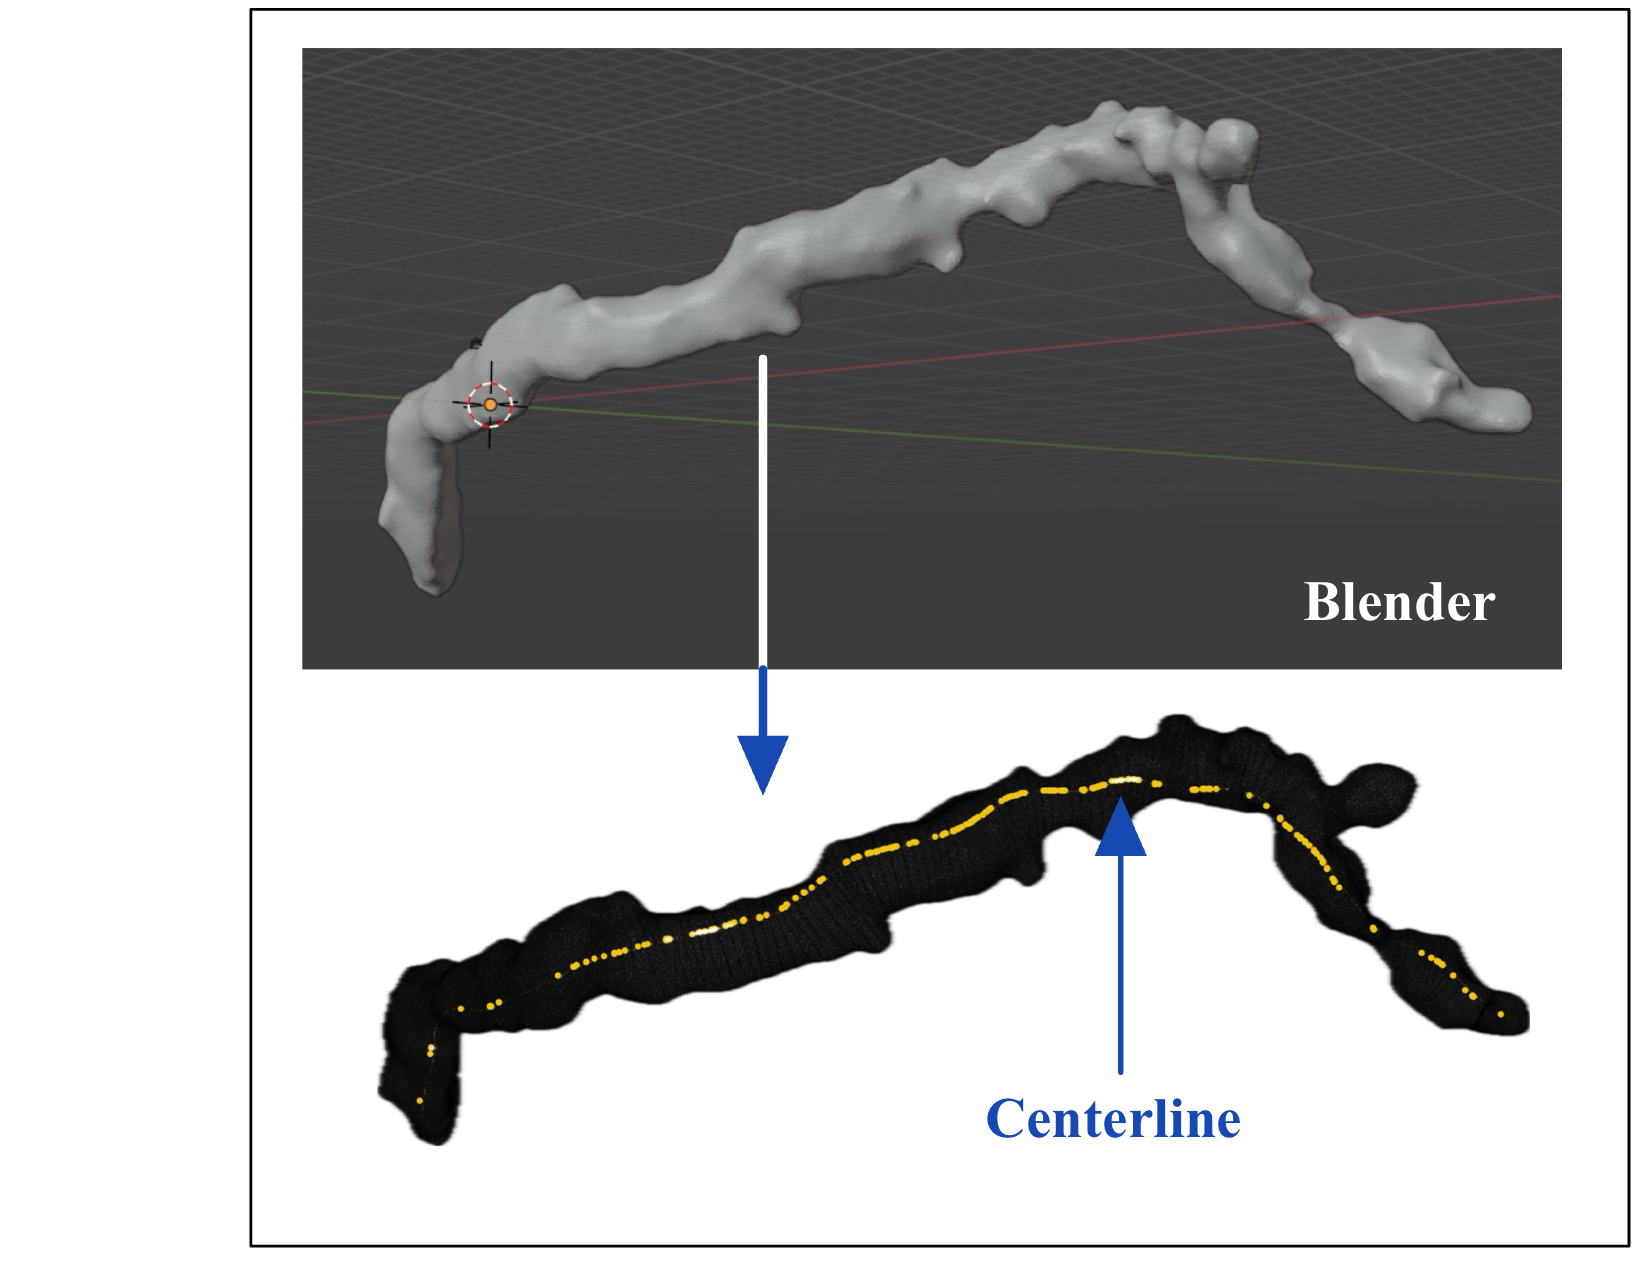
\includegraphics[width=\textwidth]{figures/Centerline.jpg}
                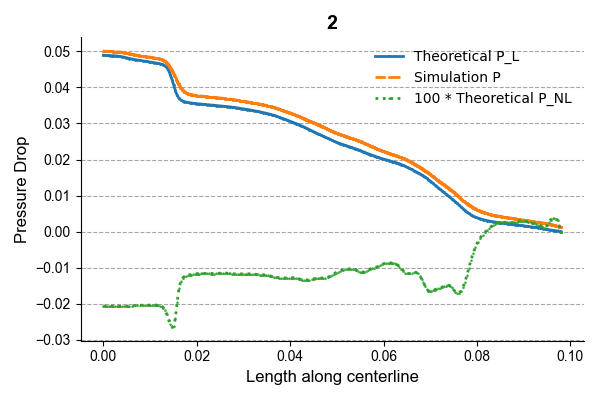
\includegraphics[width=\textwidth]{figures/Cline_2_NL.jpg}
            \end{figure}
        \end{column}

        \hspace{0.03\textwidth}

        \begin{column}{0.6\textwidth}

            Analytical Solution:


            \vspace{0.02\textwidth}


            \resizebox{\textwidth}{!}{$
            P = 
            - \left[\frac{\textcolor{red}{\alpha}}{\rho} F_{NL}(A(x), S(x))\right] \dot{m}^2 
            - \left[K_R F_{L}(A(x), S(x))\right] \dot{m}
            $}


            \vspace{0.02\textwidth}

            
            Correlation of pressure drop linear part 
            with CFD result:
            
            \begin{figure}[H]
                \centering
                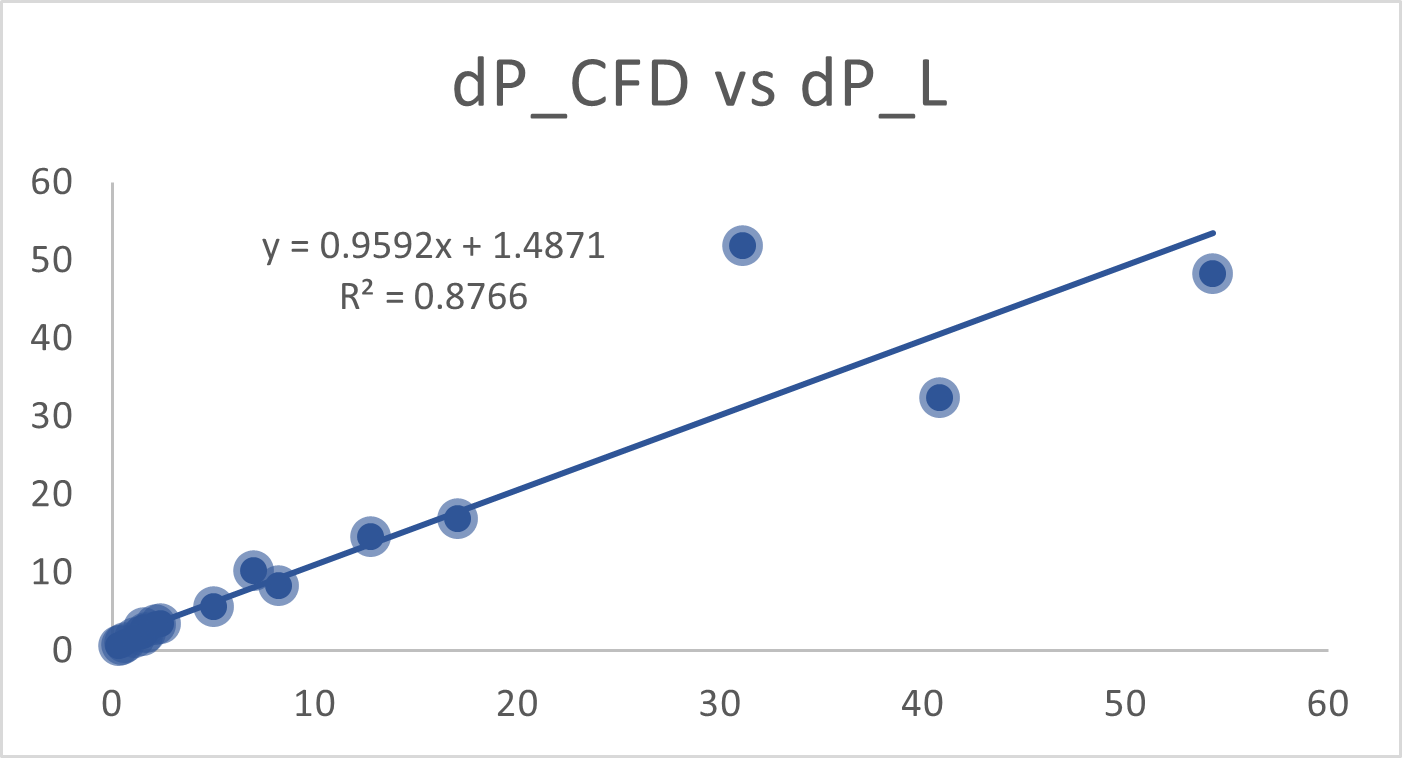
\includegraphics[width=\textwidth]{figures/Result_T.jpg}
                \caption{$dP_{CFD}$ correlation with $dP_L$ among 17 cases}
            \end{figure}

            \vspace{-0.1\textwidth}

            \begin{table}[H]
                \centering
                \resizebox{\textwidth}{!}{
                \begin{tabular}{@{} l r r r r r r r r r r r r r r r r r @{}}
                \toprule
                \textbf{dP}   & \textbf{1} & \textbf{2} & \textbf{4} & \textbf{6} & \textbf{8} & \textbf{13} & \textbf{14} & \textbf{15} & \textbf{16} & \textbf{17} & \textbf{18} & \textbf{19} & \textbf{20} & \textbf{21} & \textbf{24} & \textbf{26} & \textbf{27} \\
                \midrule
                \textbf{0.01} & 20\% & 2\% & 5\% & 1\% & 25\% & 15\% & 39\% & 11\% & -43\% & 35\% & -35\% & 24\% & 16\% & -9\% & 22\% & -13\% & -2\% \\
                \textbf{0.05} & 27\% & 6\% & 25\% & 21\% & 32\% & 20\% & 43\% & 14\% & -35\% & 42\% & -23\% & 26\% & 24\% & -5\% & 27\% & -7\% & 5\% \\
                \textbf{0.1} & 33\% & 11\% & 40\% & 35\% & 38\% & 26\% & 46\% & 18\% & -26\% & 48\% & -13\% & 31\% & 31\% & 0\% & 31\% & -1\% & 13\% \\
                \bottomrule
                \end{tabular}
                }
                \caption{Origional Error of Theoretical Result}
                \label{tab:dP-analysis}
            \end{table}
                
        \end{column}

        
    \end{columns}


    

\end{frame}





% Page - Analytical Approach: Curvecture Effect %%%%%%%%%%%%%%%%%%%%%%%%%%%%%%%%%%%%%
\begin{frame}
    \fontsize{8pt}{10pt}\selectfont
    \frametitle{Analytical Approach: Curvecture Effect}

    As the curvature of the PD varies across 
    locations and differs for each case, 
    we also discussed the curvature results 
    derived from the analytical approach:

    \begin{figure}[H]
        \centering
        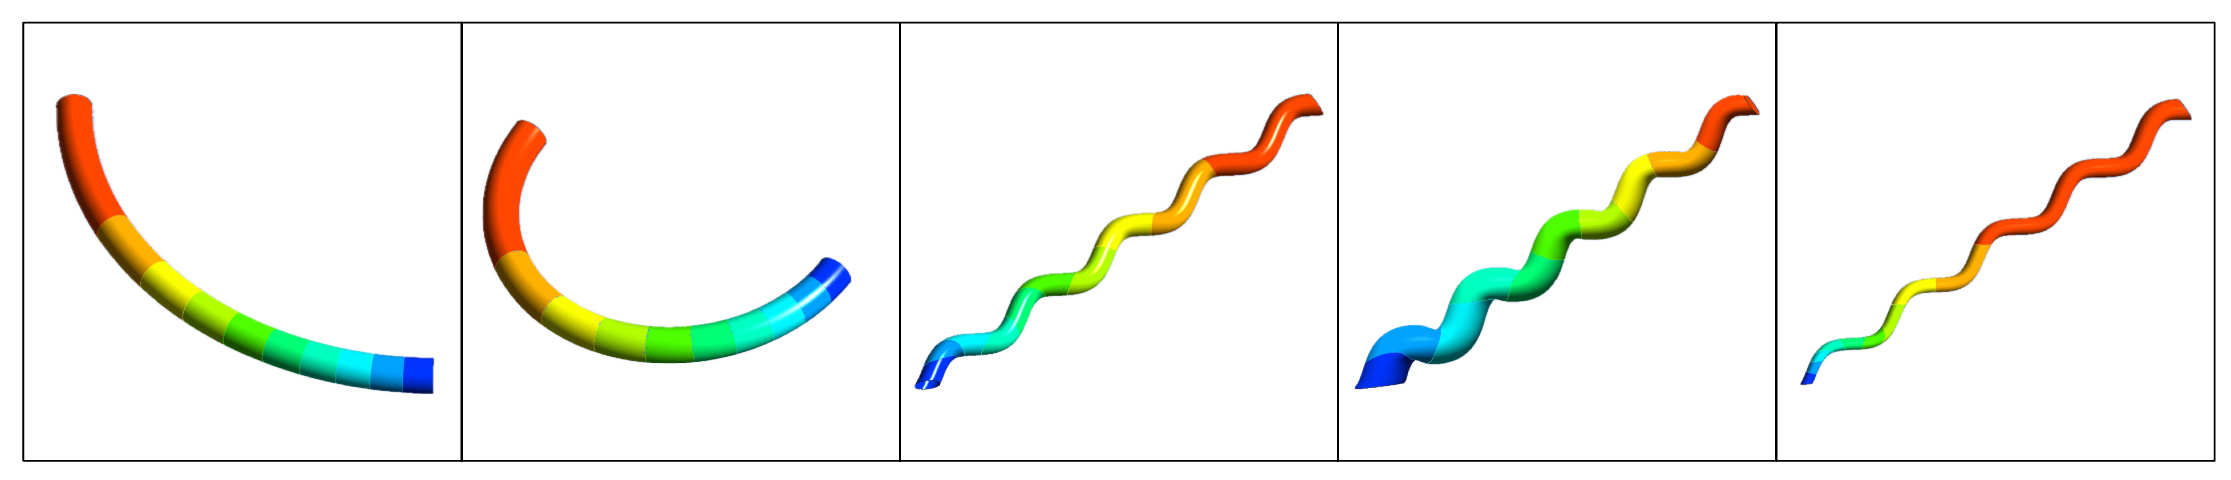
\includegraphics[width=\textwidth]{figures/Curvature.jpg}
        % \caption{$dP_{CFD}$ correlation with $dP_L$ among 17 cases}
    \end{figure}

    \begin{table}[H]
        \centering
        \resizebox{\textwidth}{!}{
        \begin{tabular}{l c c c c c}
        \toprule
        \textbf{$\dot{M}$} & \textbf{90-degree-pipe} & \textbf{180-degree-pipe} & \textbf{sin-curved-pipe} & \textbf{sin-dilation-pipe} & \textbf{sin-structure-pipe} \\
        \midrule
        0.01 & 12\%  & 2\%   & -7\%   & -14\%  & 7\%   \\
        0.05 & 6\%   & -2\%  & -12\%  & -17\%  & -2\%  \\
        0.1  & 0\%   & -8\%  & -18\%  & -20\%  & -12\% \\
        0.2  & -11\% & -18\% & -29\%  & -28\%  & -28\% \\
        \bottomrule
        \end{tabular}
        }
        \label{tab:error-percentages-transposed}
        \end{table}

        We observed that the Sin-dilation pipe 
        exhibits the largest error among different
         mass sources. 


         \vspace{0.02\textwidth}
         
         
         Which may suggest that, in \textbf{low-pressure drop 
         scenarios, curvature could have a greater i
         nfluence} on the error in the analytical approach.
    


    
\end{frame}






% Page - Analytical Approach: Road Map For Next Step  %%%%%%%%%%%%%%%%%%%%%%%%%%%%%%%%%%%%%
\begin{frame}
    \fontsize{8pt}{10pt}\selectfont
    \frametitle{Analytical Approach: Road Map For Pressure Prediction }

    As we already have PD strcuture parameters,
    linear and non-linear term dP result, and CFD
    dP result,
    next phase is to deploy PINN to obtain 
    pressure drop prediction:
    \begin{figure}[H]
        \centering
        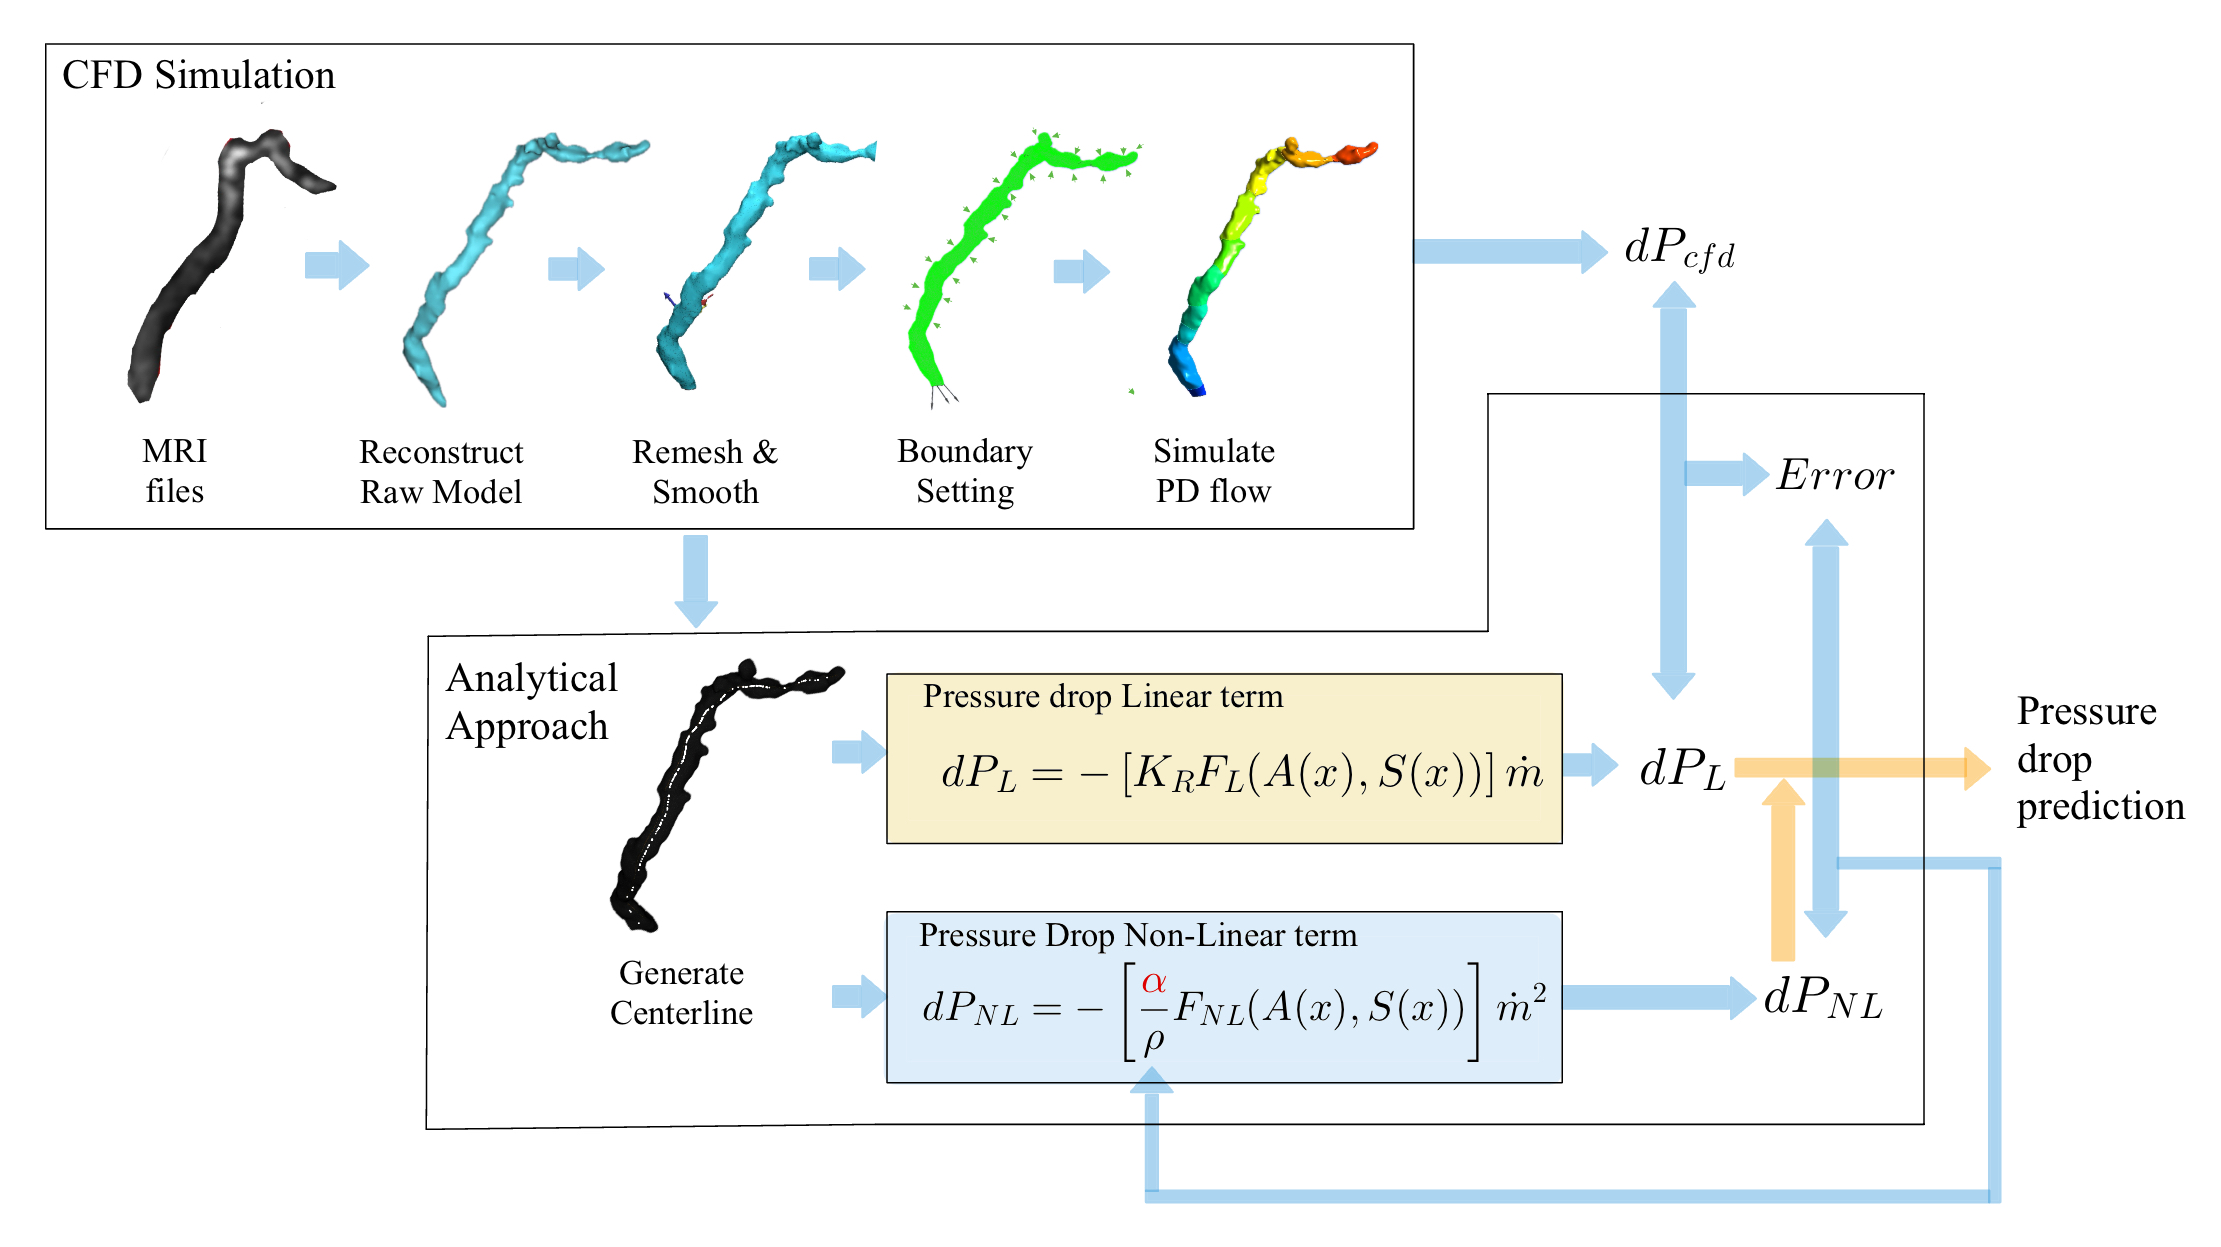
\includegraphics[width=\textwidth]{figures/Process-Total.jpg}
        \caption{\footnotesize{Road map for pressure prediction \\
            Blue arrow: internal calculation and $\alpha$ iteration \\
            Orange arrow: Obtain Prediction}
        }
    \end{figure}

    
\end{frame}








% Page - Myself  %%%%%%%%%%%%%%%%%%%%%%%%%%%%%%%%%%%%%
\begin{frame}
    \fontsize{8pt}{10pt}\selectfont
    \frametitle{Speaker Info }


    Personal Website Link: \href{https://zhbalex.github.io}{https://zhbalex.github.io}


    \begin{figure}[H]
        \centering
        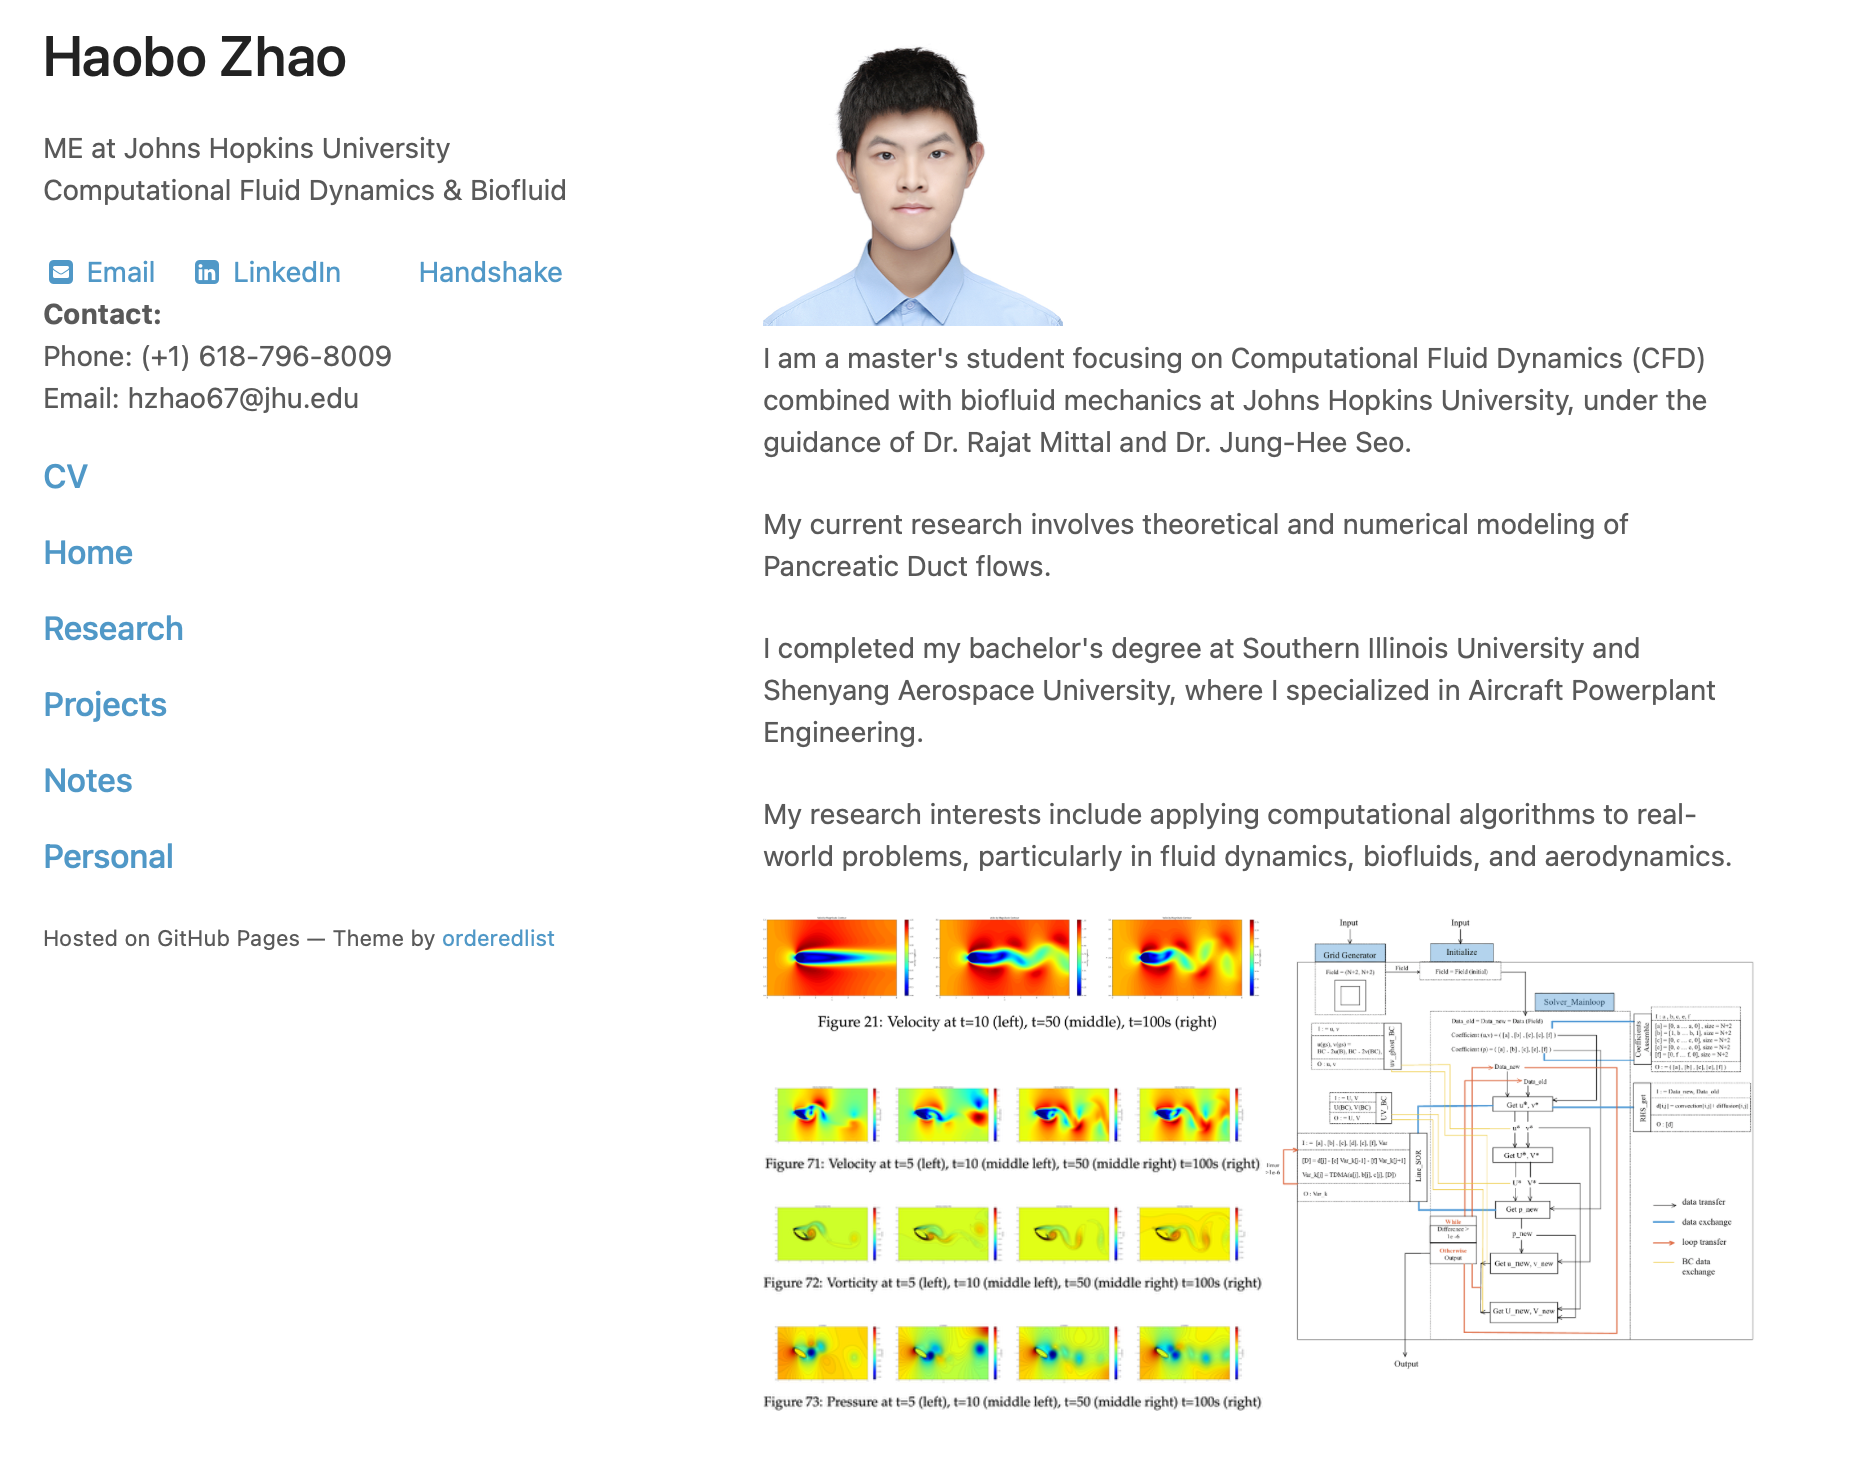
\includegraphics[width=0.8\textwidth]{figures/Speaker_info.jpg}

    \end{figure}



    
\end{frame}
















\end{document}